\documentclass[12pt,a4paper]{report}

% Start document preamble.
% The fullpage package sets up the margin for the entire document.
\usepackage{fullpage}
% \usepackage{geometry}
% \geometry{a4paper, margin=0.9in}

% For image and graphics support.
\usepackage{graphics}
\usepackage{epsf,graphicx}
\usepackage[framemethod=tikz]{mdframed}

\mdfdefinestyle{mystyle}{%
  rightline=true,
  innerleftmargin=10,
  innerrightmargin=10,
  outerlinewidth=3pt,
  topline=false,
  rightline=true,
  bottomline=false,
  skipabove=\topsep,
  skipbelow=\topsep
}

% To use a different bibliography style, just change "numeric" to
% your preferred style (mla for MLA style, alphabetic for Author-Year
% style, etc.) There are a lot of options; check the BibLaTeX documentation.
\usepackage[numbers, sort&compress]{natbib}
\bibliographystyle{apsrev4-2}
% \usepackage{multicol}
% \renewcommand{\bibpreamble}{\begin{multicols}{2}}
% \renewcommand{\bibpostamble}{\end{multicols}}

% The microtype package fixes a lot of small typographical things.
% They're hard to see, but your eyes will thank you!
\usepackage{microtype}

% We should support UTF-8 in the input file (since it is the twenty-first
% century, after all)
\usepackage[utf8]{inputenc}

% And we should use T1 for the output encoding, because the default results
% in a big mess with accented characters in the PDF
\usepackage[T1]{fontenc}

% The Babel package modernizes the hyphenation routines.
% Here, we configure it to use UK English.
\usepackage[british]{babel}
% \renewcommand{\bibsection}{\chapter*{References}}

% The titling package allows us to rewrite the \maketitle command easily.
\usepackage{titling}

% The setspace package lets us adjust line spacing
\usepackage{setspace}
\usepackage{xspace}

% The enumerate package is used to enhance enumerated lists
\usepackage{enumerate}

% The csquotes package provides nice facilities for quotations.
\usepackage[babel]{csquotes}

% The amsthm package lets us set up theorem-like environments
\usepackage{amsthm}
\usepackage{amsmath}
% \usepackage{physics} % I dislike this package a bit, so not using it.

% The mathtools and amssymb packages provide some important mathematical support
\usepackage{amsfonts, amssymb, mathtools, amstext}
\usepackage{bm}

% The booktabs package facilitates high-quality table formatting.
\usepackage{booktabs}
\usepackage{setspace}

\usepackage{listings}
\usepackage{xcolor}

\definecolor{codegreen}{rgb}{0,0.6,0}
\definecolor{codegray}{rgb}{0.5,0.5,0.5}
\definecolor{codepurple}{rgb}{0.58,0,0.82}
\definecolor{backcolour}{rgb}{0.95,0.95,0.92}

\lstdefinestyle{mystyle}{
    backgroundcolor=\color{backcolour},   
    commentstyle=\color{codegreen},
    keywordstyle=\color{magenta},
    numberstyle=\tiny\color{codegray},
    stringstyle=\color{codepurple},
    basicstyle=\ttfamily\footnotesize,
    breakatwhitespace=false,         
    breaklines=true,                 
    captionpos=b,                    
    keepspaces=true,                 
    numbers=left,                    
    numbersep=5pt,                  
    showspaces=false,                
    showstringspaces=false,
    showtabs=false,                  
    tabsize=2
}

\lstset{style=mystyle}

% The hyperref package sets up PDF hyperlinks and other fanciness.
% WARNING: THIS MUST BE THE LAST PACKAGE LOAD
\usepackage{url}
\usepackage{hyperref}

% The cleveref package handles a lot of fanciness with internal cross-references.
% Curiously, it has to come *after* hyperref.
\usepackage[capitalize]{cleveref}
\crefname{equation}{equation}{equations}
\Crefname{equation}{Equation}{Equations}

%% DEFINE COMMANDS

% We create some theorem-like environments
\theoremstyle{plain}
\newtheorem{theorem}{Theorem}[section]
\newtheorem{corollary}[theorem]{Corollary}
\newtheorem{lemma}[theorem]{Lemma}
\newtheorem{proposition}[theorem]{Proposition}
\newtheorem{observation}[theorem]{Observation}

\newtheorem*{theorem*}{Theorem}
\newtheorem*{corollary*}{Corollary}
\newtheorem*{lemma*}{Lemma}
\newtheorem*{proposition*}{Proposition}
\newtheorem*{observation*}{Observation}

\theoremstyle{definition}
\newtheorem{definition}[theorem]{Definition}
\newtheorem*{definition*}{Definition}

\theoremstyle{remark}
\newtheorem{remark}[theorem]{Remark}
\newtheorem*{remark*}{Remark}

\newtheorem{example}[theorem]{Example}
\newtheorem*{example*}{Example}

\newtheorem{note}[theorem]{Note}
\newtheorem*{note*}{Note}

% The mathtools package provides facilities for many mathematical tasks.
% In particular, it sets up nice commands for formatting braces.
\DeclarePairedDelimiter{\pbrac}{(}{)}
\DeclarePairedDelimiter{\sbrac}{[}{]}
\DeclarePairedDelimiter{\cbrac}{\{}{\}}
\DeclarePairedDelimiter{\floor}{\lfloor}{\rfloor}
\DeclarePairedDelimiter{\ceil}{\lceil}{\rceil}

% Custom physics notation and shorthands because I am tired of repeating it
% everywhere.
\newcommand{\mink}{\eta_{\mu\nu}}
\renewcommand{\dag}{\dagger}
\newcommand{\munu}{\mu\nu}
\newcommand{\Hint}{\hat{H}_{\text{int}}}
\newcommand{\Hab}{\hat{H}_{AB}}
\newcommand{\ahat}{\hat{a}}
\newcommand{\bhat}{\hat{b}}
\newcommand{\g}{\mathfrak{g}}
\newcommand{\BigO}{\mathcal{O}}

% The bra and ket notation.
\DeclarePairedDelimiter\bra{\langle}{\rvert}
\DeclarePairedDelimiter\ket{\lvert}{\rangle}
\DeclarePairedDelimiterX\braket[2]{\langle}{\rangle}{#1 \delimsize\vert #2}

% Some common matrix notations.
\DeclareMathOperator{\Tr}{Tr}
\DeclareMathOperator{\diag}{diag}

% Preamble end. Begin Dissertation document.
\begin{document}

\thispagestyle{empty}

%
%	This is a basic LaTeX Template for the TP/MP MSc Dissertation report

\parindent=0pt          %  Switch off indent of paragraphs 
\parskip=5pt            %  Put 5pt between each paragraph  

%	This section generates a title page
%       Edit only the sections indicated to put in the project title, and submission date

\vspace*{0.1\textheight}

\begin{center}
        \huge{\bfseries Bridging Gravity and Quantum Mechanics: A Study of Gravitationally Induced Entanglement}\\ Draft Chapters% Replace with the title of your dissertation!
\end{center}

% \begin{center}
%         \huge{\bfseries A Brief Treatise on Gravitationally Induced Quantum Entanglement}\\ Draft Chapters% Replace with the title of your dissertation!
% \end{center}

\medskip

\begin{center}
        \Large{Prateek Gupta}\\  % Author of dissertation - replace with your name!
        \medskip
        \large{\today}  % Submission date
\end{center}

%%% If necessary, reduce the number 0.4 below so the University Crest
%%% and the words below it fit on the page.
%%% Don't let the crest, or the wording below it, flow onto the next page!

\vspace*{0.25\textheight}

\begin{center}
        
\includegraphics[width=35mm]{crest.pdf}
\end{center}

\medskip

\begin{center}

%%%
%%% Change Theoretical to Mathematical if appropriate
%%%
\large{
  MSc in Theoretical Physics\\[0.8ex]
  The University of Edinburgh\\[0.8ex]
  2023}

\end{center}
\newpage
\pagenumbering{roman}

\begin{abstract}
This is where you summarise the contents of your dissertation. It should be
at least 100 words, but not more than 250 words.
\end{abstract}

\pagenumbering{roman}

\begin{center}
\textbf{Declaration}
\end{center}

I declare that this dissertation was composed entirely by myself.

Chapters 1 and 2 provide an introduction to the subject area and a
description of previous work on this topic. They do not contain
original research.

Chapter 3 describes work that was carried out entirely by me. The results of this chapter were previously carried out by Professor Suraj N. Gupta of the University of Manchester in 1952, but the results are modified to correspond with the metric adopted in this dissertation. Few of the other results were previously obtained by Professor Marios Christodoulou of the Austrian Academy of Sciences and the University of Vienna. 

Chapter 4 and 5 describes work that was carried out entirely by me. Some of the results of this chapter have been obtained previously by Professor Sougato Bose of University College London, but our results vary slightly.

Chapters 4 also contains my original work. This original work in
Chapter 4 was carried out in collaboration with Dr Suddhasattwa Brahma.

All calculations were done by hand. Jupyter, NumPy, SciPy and matplotlib packages of Python were used to visualize some of the results.

\newpage

\begin{center}
\textbf{Personal Statement}
\end{center}

This project began with an introduction to entanglement and gravity, with my main sources being S. Bose's ``Spin Entanglement Witness for Quantum Gravity'', ``Mechanism for the Quantum Natured Gravitons to Entangle Masses'', and M. Christodoulou's ``Locally Mediated Entanglement in Linearised Quantum Gravity''. I read the first paper, and acquainted myself with the experimental setup and the thought experiments.

Once I was comfortable with that, I moved to S. Bose's second paper, where I spent some time understanding how gravity was quantised, as the paper presented a mechanism for entanglement in a perturbative setting.

The next thing I worked on was reproducing the results from the second paper, before moving to original work. The goal was to understand how they calculated Concurrence, a measure of entanglement, and how the formalism worked.

The third stage of our project was to calculate Entanglement Entropy, another measure for Entanglement, and corroborate my results with those found using Concurrence. The second and third steps took the most time as I ran into some discrepancies that I had to sort out.

The fourth and final stage of my project was to reproduce the results of M. Christodoulou's ``Locally Mediated Entanglement in Linearised Quantum Gravity,'' and try and understand how we could obtain our interaction Hamiltonian from first principles, and deepen my understanding of how first principles can be used to derive the Newtonian potential between $N$ point masses covariantly.

During the course of the project, I met with my supervisor roughly every week,
in order to discuss my progress and the direction I would head
next.

I started writing this dissertation in around the end of July, and I spent the first
three weeks of August working on it full-time.

Overall, I feel that the project was a success, and I found it to be
extremely enjoyable throughout.


\newpage

\begin{center}
%\vspace*{2in}
% an acknowledgements section is completely optional but if you decide
% not to include it you should still include an empty {titlepage}
% environment as this initialises things like section and page numbering.
\textbf{Acknowledgements}
\end{center}

I'd like to thank my supervisor Dr Suddhasattwa Brahma for
making this project possible, and for his immense patience and his detailed functional explanations of the thought experiments and mathematical expertise. Thanks also to my fellow MSc student Han Wang, also working under the supervision of Dr. Brahma on a similar topic, for being a sounding board for some of my ideas.

I would also like to thank my fellow MSc students Maegan Anderson and Joe Milarvie for their various inputs throughout the dissertation process.

The document was typeset using \LaTeX\ and the template for this document was provided by the School of Physics for MSc Theoretical Physics.

\newpage
\tableofcontents
\newpage
\listoffigures

\newpage
\pagenumbering{arabic}
\chapter{Introduction}

To talk about quantum gravity, I will start with the story about the clash between General Relativity and Quantum Mechanics and how it gave birth to one of the biggest crises known to Physics.

Ten years after Einstein shook the world with the \textit{Annus Mirabilis} papers, which gave the world the Theory of Special Relativity and the world-famous equation for mass-energy equivalence, $E = mc^2$, he shocked the world of physics once again with his General Theory of Relativity, in a series of papers published in 1915. Furthermore, by the end of 1915, he published the Field Equations of Gravity, providing a description of gravity as a geometric property of space and time and how the curvature of the four-dimensional spacetime was directly related to the energy and momentum of matter and radiation \cite{EinsteinFieldEq}. And thus, we had the first classical field theory of gravity. This also forms the basis of the Standard Model of Cosmology we use today.

Around the same time, a group of physicists which included the likes of Max Born, Werner Heisenberg and Wolfgang Pauli, made great strides in the field of quantum mechanics, which govern the mechanics of sub-atomic particles \cite{BornQM, BornHeisen}. However, by the mid-1920s, they hit a seemingly insurmountable problem: quantising the electromagnetic field. They found that to quantise electromagnetism correctly, and they had to quantise the classical field theory of electromagnetism \cite{PauliQE}. Furthermore, since the field equations could be rewritten using Einstein's Relativity theory, they had to incorporate special relativity into their work. Thus, the framework of Quantum Field Theory was born, and by 1927, Paul Dirac published the first theory of Quantum Electrodynamics or QED \cite{DiracFirstQED}. 

Nevertheless, as in any developmental story of a theory, they found more problems. One such problem was the problem of infinities. In the early 1930s, Robert Oppenheimer showed that higher-order perturbative calculations of QED always resulted in infinite values, such as the electron self-energy, which is the energy of the electron had as a result of changes that it causes in its environment, or the vacuum zero point energy of photon and electrons \cite{Oppie}. Thus, in the 1950s, the concept of renormalisation was introduced by Richard Feynman, Shinichiro Tomonaga \cite{Tomonaga1948OnIF, Fukuda1948ASS}, Julian Schwinger \cite{PhysRev.74.1439}, and Freeman Dyson, for which the first three of them even jointly won the Nobel Prize in Physics \cite{Schweber1994QEDAT}. This framework allowed them to eliminate the problem of infinities in perturbative quantum field theory, and we finally had a more complete theory of Quantum Electrodynamics. 

Thus, the field of Quantum Field Theory boomed. Physicists formulated a quantum field theory of the strong force, which they named Quantum Chromodynamics, unified the Weak and Electromagnetic forces, and theorised the Higgs Mechanism. Furthermore, by the 1970s, they formulated a Standard Model of Particle Physics incorporating all of these theories, and we now had a model where three of the four fundamental forces were governed by the laws of Quantum Field Theory.

Surely, physicists thought at the time, if Quantum Field Theory could describe three of the four fundamental forces, the final known fundamental force, gravity, would be no different. They thought that finally, finally, they could grasp a Unified Theory which could explain everything. Thus, Einstein's field theory equations, published in 1915, met the new and improved framework of Quantum Field Theory. However, as always, luck was not on the side of the physicists. It turned out that Einstein's Field Theory for Gravity was extraordinarily incompatible with the framework of Quantum Field Theory. Not only did classical General Relativity have singularities, like singularities in Black Holes and the Big Bang singularity, but it also had UV behaviour near Planck scales. 

However, the biggest of these problems was that the field equations had a coupling with units, $G_N$, which made the field equations utterly non-renormalisable, and without renormalizability, a quantum field theory could not be generated. Several theories have been proposed to circumvent or counter this. Examples include String Theory, a framework in which the point-like particles are replaced by one-dimensional objects called strings \cite{Tong_2009}; Loop Quantum Gravity; Supergravity, which employs the framework of Superstring theory; or Double Copy Theory, which hypothesises a perturbative duality between gauge theory and gravity \cite{DoubleCopy}. Moreover, many of these theories are highly untestable by experiments or have huge inconsistencies which are yet to be resolved.

Even then, one could say that General Relativity contains the seeds of its own destruction \cite{Tong_2009}. We can say that the singularities, the UV behaviour, and the non-renormalizability are all \textit{known} unknowns or known problems that need to be solved for a theory of quantum gravity. However, the theory could host several \textit{unknown} unknowns, problems we did not even know existed. One such problem, as some physicists have pointed out, mainly because of the lack of experiments, is the question about the nature of gravity itself. Is gravity even quantisable in the first place? Does it even have a quantum nature? Because if it is not quantisable and does not have a quantum nature, we must look into different theories to resolve the problems of singularities and divergent behaviour of General Relativity.

To this end, many physicists in the 21st Century have developed various gedankenexperiments \cite{PhysRevD.98.126009, doi:10.1142/S0218271819430016}, or thought experiments, and tabletop experiments. I will briefly introduce one such experiment called the Bose-Marletto-Vedral (BMV) \cite{Bose_2017, Marletto_2017} experiment in the next chapter, but the main feature of many of these experiments, including the BMV experiment, include entanglement due to gravitational interactions. This is because all quantum interactions induce entanglement, as I will also show in the next chapter. And if gravity can induce entanglement, then indeed, one could say with some certainty that gravity has a quantum nature.

In this dissertation, I will first explain the conceptual underpinnings of the BMV experiment, and how it uses a few central principles of Quantum Information Theory, how quantum interactions can induce entanglement within a system of two quantum harmonic oscillators, and how to calculate two separate measures of entanglement called Concurrence and Entanglement Entropy \cite{Bose_2022}. I will then briefly describe how one can linearise Einstein's Field equations and then quantise them using canonical quantisation \cite{Gupta_1952}. I will also describe how we could use this quantisation as a driving force for the interaction between the quantum oscillators.

I will also show how we can derive the same interaction Hamiltonian from first principles and how the slow-motion approximation of the action for an $N$ point masses would yield an action with potential energy similar to that of a Newtonian gravitational potential energy \cite{Christodoulou_2023b}.

I will then go back and describe a proposed mechanism for gravity to entangle the two quantum harmonic oscillators and show that if we were to calculate a shift in the energy of the quantised graviton from the earlier canonical quantisation is also the same as the Newtonian gravitational potential energy between two bodies. I will then derive the concurrence \cite{Bose_2022} and entanglement entropy, the two measures of entanglement, for these interactions. Then, I will analyse the results in more depth and look at the analytical and numerical behaviour.

Finally, I will conclude with the implications and summary of the results and potential experiments that one can conduct to see evidence of this mechanism and the consequences of these results for the story of quantum gravity.

\newpage
\chapter{Background Theory}
\section{Quantum Entanglement and the BMV Experiment}
Before getting into the theory behind the BMV Experiment, let us first define Quantum Entanglement. Quantum Entanglement is defined as the phenomenon where a pair of particles interact in a way such that the state of each particle cannot be described independently of the state of the other, even if they are at large distances \cite{schrodinger_1935}. Erwin Schr\"odinger defined this as the \textit{characteristic} trait of a quantum interaction \cite{schrodinger_1935}. 

As stated before, due to the lack of evidence for quantum aspects, there is a great debate about the nature of gravity \cite{Bose_2017, fdysongraviton}. Some even use the breakdown of quantum mechanics itself at massive scales capable of producing gravitational effects to justify that gravity need not be a quantised field \cite{penrose}. A few of the proposed tests aimed at probing this question of gravity's quantum nature have traditionally focused on phenomenology and cosmological observations \cite{Bose_2017, Hossenfelder_2012}. However, \citet{Bose_2017} and \citet{Marletto_2017} opened up a different avenue to study the same question: probing the quantum coherent aspect of gravity, which seems to offer a much more prominent and unambiguous witness to quantum gravity \cite{Bose_2017}.

In the same spirit as a Bell inequality certifies the ``non-local'' character of quantum mechanics \cite{Bell}, the BMV thought experiment shows that the growth of entanglement between two mesoscopic masses held in a superposition  of spatially localised states $\ket{L}$ and $\ket{R}$ (as shown in Fig. \ref{fig:BMV}(a)\cite{Bose_2017}), say in adjacent wave-matter interferometers as shown in Fig \ref{fig:BMV}(b\cite{Bose_2017}, can be used to certify the quantum nature of gravitational interactions.

The proposal relies on the assumption that the gravitational interaction between the two masses is mediated by a gravitational field, and there are no other forces, like the short range Casimir-Polder force, in play. Upon making this assumption, the proposal borrows and uses a central principle of Quantum Information Theory, that entanglement between two systems \textit{cannot} be created by Local Operations and Classical Communications (LOCC) \cite{RevModPhys.81.865}. Here, ``Local Operations" means that the two subsystems are each allowed to do anything allowed by quantum mechanics to their subsystem but nothing that requires an interaction between them. ``Classical Communication" means the subsystems ``communicate" through a classical channel \cite{Bose_2017}. 

\begin{figure}[ht!]
    \centering
    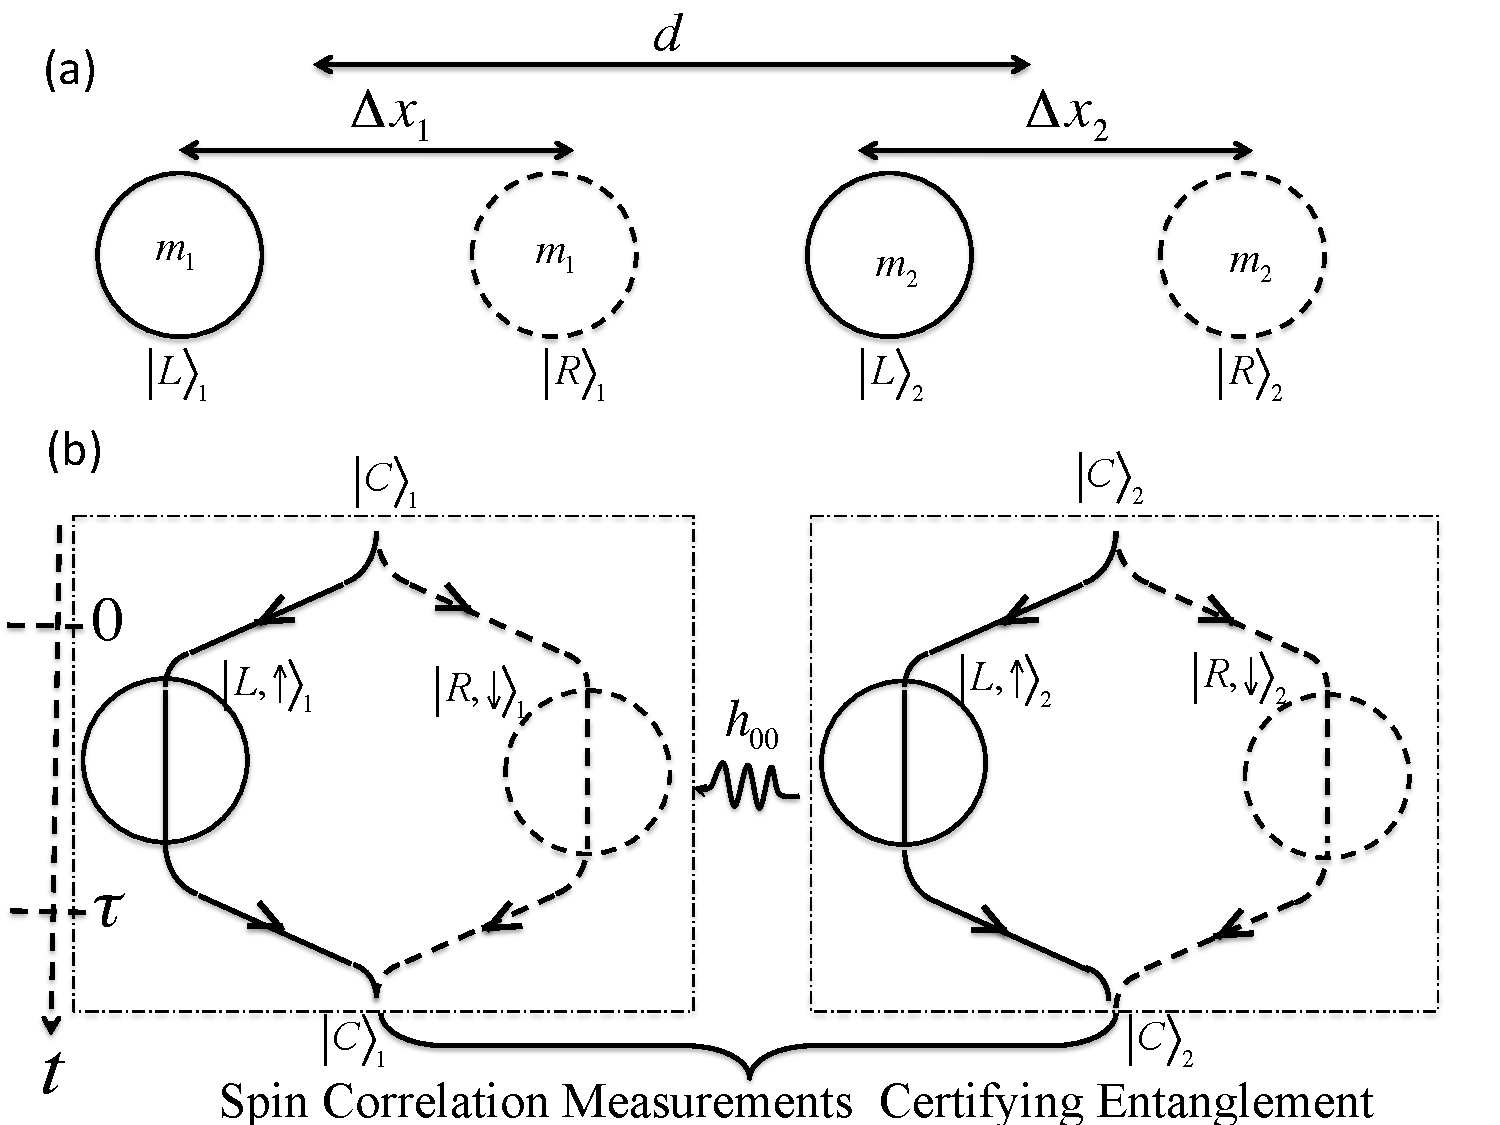
\includegraphics[width=10cm]{LR_fig.pdf}
    \caption{Schematic Diagrams for the BMV Experiment.}
    \label{fig:BMV}
\end{figure}

It can be proved that in the absence of closed timelike loops \cite{timelike} and under the assumption of validity of the chronology protection conjecture \cite{PhysRevLett.68.267}, as long as the notion of classicity itself is not extended \cite{Hall_2018}, LOCC keeps any initially unentangled state separable \cite{Bose_2017}. If gravitational interactions entangle the masses, the entanglement must have occurred through local operations and ``quantum" communication (LOQC), where ``quantum" is essentially anything that does not fall under the aforementioned notion of classicity. That is, if mutual gravitational interaction between two masses entangles them, then the mediating gravitational field is \textit{necessarily} quantum mechanical in nature \cite{Bose_2017}.

 Consider now, the schematic version presented in Fig \ref{fig:BMV}(a). Two neutral test masses $m_1$ and $m_2$ are held steadily in a superposition of two spatially separated states $|L\rangle$ and  $|R\rangle$, whose centres are separated by a distance $\Delta x$ and each state is a localised Gaussian wave packet with small enough width to assume $\langle L|R\rangle = 0$. There is a separation $d$ between the centres of the superpositions so that the short range Casimir-Polder force is negligible even at the closest approach of the masses. As the masses are separated by different distances, distinct components of the superposition have distinct gravitational interaction energies and thus have different rates of phase evolution. Therefore the time evolution of the joint state of the two masses is purely due to gravitational interactions between them \cite{Bose_2017}.

Fig \ref{fig:BMV}(b) shows the Stern-Gerlach (SG) interferometry which includes three steps: (1) A spin dependent spatial splitting of the centre of mass state of a test mass in an inhomogenous magnetic field, (2) ``Holding" the coherent superposition created above for a time $\tau$, where the magnetic field of the SG is effectively turned off and finally (3) bring back the superposition through unitary transformations. If the state is proven to be entangled, then the mediator, the gravitational field, is a quantum entity. A more detailed scheme is presented in \citet{Bose_2017}.

I have now explained the conceptual theory behind the BMV experiment. Detailed information and a nice review about this experiment and its workings, as well as the demanding nature of this experiment, can be found in a separate work done by Han Wang \cite{han} for his Master's dissertation (submitted 2023), and in \citet{Christodoulou_2020}. The main focus of this dissertation is the review and analysis of the concepts behind gravitationally induced entanglement using these concepts.

\section{Entanglement Due to Quantum Interactions} \label{sec: QHOs}
Let us now look at quantum interactions and how they induce entanglement. Consider a setup of two Quantum Harmonic Oscillators (QHOs) in the presence of a gravitational field, denoted by A and B, located at $\pm d/2$. Assume that the harmonic oscillators are well-localised, such that,

\begin{equation}
    \hat{x}_{A}=-\frac{d}{2}+\delta\hat{x}_{A},\qquad \hat{x}_{B}=\frac{d}{2}+\delta\hat{x}_{B},
    \label{eq: Oscillator Locations}
\end{equation}

where $\hat{x}_{A}$, $\hat{x}_{B}$ are the positions, and $\delta\hat{x}_{A}$, $\delta\hat{x}_{B}$ denote small displacements from the equilibrium. Thus the Hamiltonian for the two QHOs is given by \cite{Bose_2022,griffiths_schroeter_2018,Tannoudji_2019},

\begin{equation}
    \hat{H}_{\text{matter}} =  \frac{\hat{p}_A^2}{2m} + \frac{\hat{p}_B^2}{2m} + \frac{m\omega_m^2}{2}\delta\hat{x}^2_{A} + \frac{m\omega_m^2}{2}\delta\hat{x}^2_{B},
\end{equation}

where $\hat{p}_A$ and $\hat{p}_B$ are the conjugate momenta, and $\omega_m$ is the harmonic frequency of the QHOs. We will assume, for simplicity, that the aforementioned frequency is equal for both QHOs. Then, the mode operators can be introduced using,

\begin{equation} \label{eq: ModeOp1}
    \delta\hat{x}_{A} = \sqrt{\frac{\hbar}{2m\omega_m}}(\hat{a} + \hat{a}^{\dag}), \qquad \delta\hat{x}_{B} = \sqrt{\frac{\hbar}{2m\omega_m}}(\hat{b} + \hat{b}^{\dag}),
\end{equation}
\begin{equation} \label{eq: ModeOp2}
    \hat{p}_A = i\sqrt{\frac{\hbar m\omega_m}{2}}(\hat{a} - \hat{a}^{\dag}), \qquad \hat{p}_B = i\sqrt{\frac{\hbar m\omega_m}{2}}(\hat{b} - \hat{b}^{\dag}),
\end{equation}

where the mode operators follow the usual commutation relations $[\hat{a}, \hat{a}^{\dag}] = 1$ and $[\hat{b}, \hat{b}^{\dag}] = 1$. These results and derivations can be found in any introductory quantum mechanics textbook such as \citet{griffiths_schroeter_2018} and \citet{Tannoudji_2019}. Thus, the Hamiltonian can be written as,
\begin{equation}
    \hat{H}_{\text{matter}} = \hat{H}_A + \hat{H}_B,
\end{equation}

where $\hat{H}_A = \hbar\omega_m \hat{a}^{\dag}\hat{a}$, and $\hat{H}_B = \hbar\omega_m \hat{b}^{\dag}\hat{b}$.

Let us now investigate the initial state of the matter system when perturbed by an interaction Hamiltonian $H_{AB}$.

Let us assume that the initial state of the matter system is given by,
\begin{equation}
    \ket{\psi_i} = \ket{0}_A\ket{0}_B,
    \label{eq: UnperturbedState}
\end{equation}
where $\ket{0}_A$ and $\ket{0}_B$ denote the ground state of the first and second  QHOs respectively. In future equations, we will use this same order, and omit the subscripts for ease of notation.

Suppose a perturbation is introduced using an interaction potential $\lambda H_{AB}$, where $\lambda$ is a small parameter, between the two systems. Then the perturbed state is given by,
\begin{equation}
    \ket{\psi_f} = \frac{1}{\sqrt{\mathcal{N}}} \sum_{n,N} C_{nN} \ket{n}\ket{N} 
    \label{eq: FinalState}
\end{equation}
where $\ket{n}, \ket{N}$ denote number states of A and B respectively, while $\mathcal{N}$ is the normalisation given by $\mathcal{N} = \sum_{n,N} |C_{nN}|^2$. We know from Eq. \ref{eq: UnperturbedState} that the coefficient of the unperturbed state is $C_{00} = 1$. The remaining coefficients are given by \cite{Bose_2022, Bala_2012},
\begin{equation}
    C_{nN} = \lambda\frac{\bra{n}\bra{N}\hat{H}_{AB}\ket{0}\ket{0}}{2E_0 - E_n - E_N},
    \label{eq: CoeffCalc}
\end{equation}
where $E_0$ is the ground state (assumed to be the same for both systems for simplicity), and $E_n$ and $E_N$ are the excited state energies. Note that the role of $\hat{H}_{AB}$ is that of a quantum operator. Were it to be a classical operator, then in Eq. \ref{eq: CoeffCalc}, it would be a complex number which would come out of the inner product thus giving us $\braket{n, N}{0, 0}$, which would give us zero by the orthogonality of the states for $n, N > 0$. Thus the coefficients would all be zero for $n,N > 0$ and the quantum state would \textit{remain unperturbed} by the classical interaction potential. Alternatively, we can say that now the difference between LOQC and LOCC is encoded in $\hat{H}_{AB}$.

If we set $A_n \equiv C_{n0}$ and $B_N \equiv C_{0N}$, then we can write the perturbed state as \cite{Bala_2012},
\begin{equation}
    \begin{aligned}
        \ket{\psi_f} &= \frac{1}{\sqrt{\mathcal{N}}} \Bigg(\ket{0}\ket{0} + \sum_{n>0} A_n \ket{n}\ket{0} + \sum_{N>0} B_N \ket{0}\ket{N} + \sum_{n, N > 0} C_{nN} \ket{n}\ket{N}\Bigg) \\
        &= \frac{1}{\sqrt{\mathcal{N}}} \Bigg( \Big(\ket{0} + \sum_{n>0} A_n \ket{n}\Big) \ket{0} + \Big(\ket{0} + \sum_{n>0} A_n \ket{n}\Big) \sum_{N>0} B_N \ket{N}\\ &\qquad\qquad + \sum_{n, N > 0} (C_{nN} - A_nB_N) \ket{n}\ket{N} \Bigg)\\
        &= \frac{1}{\sqrt{\mathcal{N}}} \Bigg( \Big(\ket{0} + \sum_{n>0} A_n \ket{n}\Big)\Big(\ket{0} + \sum_{N>0} B_N \ket{N}\Big) + \sum_{n, N > 0} (C_{nN} - A_nB_N) \ket{n}\ket{N} \Bigg)\\
    \end{aligned}
\end{equation}
Here, the first term would yield a separable state and will not be responsible for the entanglement of the system, as interactions acting as operators on only one of the two quantum systems cannot entangle the two systems \cite{Bose_2022}. Thus the $A_n$ and $B_N$ terms will not contribute to the entanglement in first order perturbation theory. The second term in the equation is responsible for the entanglement between the two matter systems. This shows the stark difference between LOCC and LOQC as explained in the previous chapter. The non-trivial part of an LOQC mechanism encoded in the Hamiltonian produces the second term in the last line of the above equation, and LOCC can only produce the first term, not the second \cite{Bose_2022}.

To compute the degree of entanglement, one can calculate two different quantities, the \textit{Concurrence} \cite{PhysRevLett.78.5022, PhysRevA.64.042315}, and the \textit{von Neumann Entanglement Entropy} \cite{Bala_2012, PhysRevA.101.052110, suddho}.

The Concurrence is defined by \cite{PhysRevLett.78.5022, PhysRevA.64.042315},
\begin{equation}
    C \equiv \sqrt{2(1 - \Tr[\hat{\rho}_A^2])},\label{eq: Conc}
\end{equation}
where $\hat{\rho}_A$ is the density operator, and can be computed by tracing away the $B$ state as,
\begin{equation}
    \begin{aligned}
        \hat{\rho}_A &= \sum_{N} \braket{N}{\psi_f} \braket{\psi_f}{N} \\
        &= \frac{1}{\mathcal{N}} \sum_{n,n',N} C_{nN} \ket{n} \braket{N}{N} C^{*}_{n'N} \bra{n'} \braket{N}{N}  \\
        &= \frac{1}{\mathcal{N}} \sum_{n,n',N} C_{nN}C^{*}_{n'N} \ket{n}\bra{n'}
    \end{aligned}
    \label{eq: DensityMatrix}
\end{equation}
Thus the trace of $\hat{\rho}_A^2$ is given by, 
\begin{equation}
    \begin{aligned}
        \Tr[\hat{\rho}_A^2] &= \Tr\Bigg[\frac{1}{\mathcal{N}} \sum_{n,n',N} C_{nN}C^{*}_{n'N} \ket{n}\bra{n'} \frac{1}{\mathcal{N}} \sum_{n,n',N'} C_{n'N}C^{*}_{nN} \ket{n'}\bra{n}\Bigg] \\
        &= \frac{1}{\mathcal{N}^2}\sum_{n,n',N,N'} C_{nN}C^{*}_{n'N} C_{n'N'}C^{*}_{nN'}
    \end{aligned}
\end{equation}
Therefore, the concurrence is given by,
\begin{equation}
    C = \sqrt{2\bigg(1 - \frac{1}{\mathcal{N}^2}\sum_{n,n',N,N'}C_{nN}C^{*}_{n'N} C_{n'N'}C^{*}_{nN'}\bigg)}
    \label{eq: Concurrence}
\end{equation}

 As it can be seen in Eq. \ref{eq: Concurrence}, for a system with an infinite dimensional Hilbert space\footnote{Technically, the maximum of $C$ as in Eq. \ref{eq: Conc} and Eq. \ref{eq: Concurrence} depends on the minimum value of $\Tr[\hat{\rho}_A^2]$, also known as ``Purity'' of the system in Quantum Information Theory, which is dependent on the number of dimensions of the Hilbert space of the system. More on this in Chapter \ref{chap: Analysis}.}, the range for the Concurrence is $C \in [0, \sqrt{2}]$. It is $0$ for a separable state and $\sqrt{2}$ for a maximally entangled state. Similarly, for a separable state, the trace of the density operator squared will be $1$ and $0$ for a maximally entangled system.
 
The other measurement of the degree of entanglement is the von Neumann Entanglement Entropy \cite{Bala_2012, PhysRevA.101.052110, suddho}. That is given by,
\begin{equation}
    \mathcal{S}(\hat{\rho}_A) = -\Tr(\hat{\rho}_A \log{\hat{\rho}_A})
    \label{eq: Entropy}
\end{equation}
This can be calculated relatively easily by calculating the logarithm of the density operator, and remembering that for a diagonalizable matrix $M$, $\log{M} = P\log{D}P^{-1}$, and for a diagonal matrix $D$, $\log{D} = \diag(\log{d_1},\dots,\log{d_n})$.
If, in Eq. \ref{eq: CoeffCalc}, $\lambda$ is small enough, then to $\mathcal{O}(\lambda^3)$, we can calculate the von Neumann Entanglement Entropy to be \cite{Bala_2012},
\begin{equation}
    \mathcal{S}(\hat{\rho}_A) = -\lambda^2\log(\lambda^2)\sum_{n,N>0} \frac{|\bra{n}\bra{N}\hat{H}_{AB}\ket{0}\ket{0}|^2}{(2E_0 - E_n - E_N)^2} + \mathcal{O}(\lambda^3).
    \label{eq: Entropy2}
\end{equation}

Both the Concurrence and Entanglement Entropy grow as entanglement grows. In Chapter \ref{chap: Entanglement}, I will show how these quantities can be calculated in a perturbative fashion for entanglement due to gravitational interactions.

\newpage
\chapter{Quantization of Gravity and Quantum Gravitational Interactions}
In the previous chapter, we saw how quantum interactions induce entanglement. Now, we want to use gravity as the source of the quantum interaction, through a gravitational field. And as we want to consider the above setup in a gravitational field, we must first understand how the gravitational field is quantised, since we want to work in the regime of small perturbations about the Minkowski background. This section will give a brief overview of the linearization and quantization process of the gravitational field, following \citet{Gupta_1952} closely. The metric is given by $g_{\munu}$, where $\mu, \nu = 0, 1, 2, 3$ and we will use the $(-, +, +, +)$ signature throughout.\footnote{\citet{Gupta_1952} uses a slightly different signature, such that their spacetime coordinates are $(it, x_1, x_2, x_3)$. We will modify their work slightly to correspond to our chosen signature.}

\section{Linear Approximation For The Gravitational Field}
The fundamental equation for the Gravitational Field is given by Einstein's equation \cite{Gupta_1952, EinsteinGravWave},
\begin{equation}
    R^{\munu} - \frac{1}{2}Rg^{\munu} = -\frac{1}{2}\kappa^2T^{\munu},
    \label{eq: EinsteinEq}
\end{equation}
where $R^{\munu}$ and $R$ are the Ricci Tensor and Scalar respectively, $\kappa$ is a constant such that $\kappa^2 = \frac{8\pi G}{c^4}$, and $T^{\munu}$ is the Stress-Energy tensor of the matter field.

Since the covariant divergence of the Stress-Energy tensor is $0$, one can obtain an expression for the Stress-Energy tensor \textit{density} $\mathfrak{T}^{\munu} = \sqrt{-g}T^{\munu}$ (where $g$ is the determinant of the metric) \cite{Gupta_1952},
\begin{equation}
    \frac{\partial\mathfrak{T}^{\nu}_{\mu}}{\partial x^{\nu}} - \frac{1}{2}\mathfrak{T}^{\alpha\beta}\frac{\partial g_{\alpha\beta}}{\partial x^{\mu}} = 0.
    \label{eq: StEnergyDen}
\end{equation}
We can thus express the conservation of energy and momentum as,
\begin{equation}
    \frac{\partial}{\partial x^{\nu}}(\mathfrak{T}^{\nu}_{\mu} + t^{\nu}_{\mu}) = 0,
    \label{eq: PseudoStEnergyDen1}
\end{equation}
where $t^{\munu}$ is the Stress-Energy \textit{pseudo-tensor density} \cite{Gupta_1952} for the gravitational field, thus satisfying the equation,
\begin{equation}
    \frac{\partial t^{\nu}_{\mu}}{\partial x^{\nu}} = - \frac{1}{2}\mathfrak{T}^{\alpha\beta}\frac{\partial g_{\alpha\beta}}{\partial x^{\mu}}.
    \label{eq: PseudoStEnergyDen2}
\end{equation}

Following \citet{Gupta_1952} and \citet{EinsteinGravWave} we can obtain a linear approximation for the field by considering small perturbations $h_{\munu}$, where $|h_{\munu}| \ll 1$, around the Minkowski background. Thus, the metric becomes,
\begin{equation}
    g_{\munu} = \mink + h_{\munu},
\end{equation}
where $\mink = \diag(-1, +1, +1, +1)$. Then using the flat spacetime tensor notation, we can rewrite Eq. \ref{eq: EinsteinEq} and Eq. \ref{eq: PseudoStEnergyDen2} as \cite{Gupta_1952},
\begin{equation}
    \Box^2h_{\munu} - \Bigg(\frac{\partial^2h_{\mu\lambda}}{\partial x_{\nu}\partial x_{\lambda}} + \frac{\partial^2h_{\nu\lambda}}{\partial x_{\mu}\partial x_{\lambda}}\Bigg) + \frac{\partial^2h_{\lambda\lambda}}{\partial x_{\mu}\partial x_{\nu}} + \mink\Bigg(\frac{\partial^2h_{\lambda\rho}}{\partial x_{\lambda}\partial x_{\rho}} - \Box^2h_{\lambda\lambda} \Bigg) = \kappa^2T_{\munu},
    \label{eq: hEinsteinEqLong}
\end{equation}
\begin{equation}
    \frac{\partial t_{\munu}}{\partial x_{\nu}} = \frac{\kappa^2}{2}\frac{\partial h_{\nu\lambda}}{\partial x_{\mu}}T_{\nu\lambda}
    \label{eq: hAndt}
\end{equation}
where $\Box^2 = \partial^{\mu}\partial_{\mu} = \eta^{\munu}\partial_{\nu}\partial_{\mu}$.
According to \citet{EinsteinGravWave}, we can also choose coordinate/supplementary conditions given by,
\begin{equation}
    \frac{\partial h_{\munu}}{\partial x_{\nu}} -  \frac{1}{2}\frac{\partial h_{\lambda\lambda}}{\partial x_{\mu}} = 0.
    \label{eq: SuppCond1}
\end{equation}
When this condition is applied, Eq. \ref{eq: hEinsteinEqLong} reduces to,
\begin{equation}
    \Box^2h_{\munu} - \frac{1}{2}\mink\Box^2 h_{\lambda\lambda} = \kappa^2T_{\munu}.
    \label{eq: hEinsteinEqShort}
\end{equation}
It is now convenient to decompose $h_{\munu}$ as,
\begin{equation}
    h_{\munu} = \gamma_{\munu} - \frac{1}{2}\mink\gamma_{\lambda\lambda}.
\end{equation}
Thus, Eq. \ref{eq: hAndt}, Eq. \ref{eq: SuppCond1} and Eq. \ref{eq: hEinsteinEqShort} reduce to,
\begin{equation}
    \frac{\partial t_{\munu}}{\partial x_{\nu}} = \frac{\kappa^2}{2}\frac{\partial \gamma_{\nu\lambda}}{\partial x_{\mu}}T_{\nu\lambda} - \frac{\kappa^2}{4}\frac{\partial \gamma_{\lambda\lambda}}{\partial x_{\mu}}T_{\nu\nu},
    \label{eq: GammaAndt}
\end{equation}
\begin{equation}
    \frac{\partial \gamma_{\munu}}{\partial x_{\nu}} = 0,
    \label{eq: GammaSupp}
\end{equation}
\begin{equation}
    \Box^2\gamma_{\munu} = \kappa^2T_{\munu}.
    \label{eq: GammaEinstein}
\end{equation}
Thus, equations \ref{eq: GammaEinstein},\ref{eq: GammaSupp} and \ref{eq: GammaAndt} describe the linearised gravitational field \cite{Gupta_1952}. 

It should be noted that the field equation Eq. \ref{eq: GammaEinstein} and the supplementary condition Eq. \ref{eq: GammaSupp} are only compatible in an approximate sense, as they respectively give,
\begin{equation}
    \Box^2\frac{\partial\gamma_{\munu}}{\partial x_{\nu}} = \kappa^2 \frac{\partial T_{\munu}}{\partial x_nu} \qquad \text{and} \qquad \Box^2\frac{\partial\gamma_{\munu}}{\partial x_{\nu}} =  0,
\end{equation}
which are agree in the first approximation \cite{Gupta_1952}.

Thus solving for $t_{\munu}$, one gets \cite{Gupta_1952},
\begin{equation}
    t_{\munu} = \frac{1}{2}\Bigg[\frac{\partial\gamma_{\lambda\rho}}{\partial x_{\mu}}\frac{\partial\gamma_{\lambda\rho}}{\partial x_{\nu}} - \frac{1}{2}\frac{\partial\gamma_{\lambda\lambda}}{\partial x_{\mu}}\frac{\partial\gamma_{\rho\rho}}{\partial x_{\nu}} - \frac{1}{2}\mink\Bigg(\frac{\partial\gamma_{\lambda\rho}}{\partial x_{\sigma}}\frac{\partial\gamma_{\lambda\rho}}{\partial x_{\sigma}} - \frac{1}{2}\frac{\partial\gamma_{\lambda\lambda}}{\partial x_{\sigma}}\frac{\partial\gamma_{\rho\rho}}{\partial x_{\sigma}}\Bigg)\Bigg]
    \label{eq: PseudoStEnergyDen3}
\end{equation}
Thus, we can get the Hamiltonian Density as,
\begin{equation}
    H = t_{00} = \frac{1}{2}\Bigg[\frac{\partial\gamma_{\lambda\rho}}{\partial t}\frac{\partial\gamma_{\lambda\rho}}{\partial t} - \frac{1}{2}\frac{\partial\gamma_{\lambda\lambda}}{\partial t}\frac{\partial\gamma_{\rho\rho}}{\partial t} + \frac{1}{2}\Bigg(\frac{\partial\gamma_{\lambda\rho}}{\partial x_{\sigma}}\frac{\partial\gamma_{\lambda\rho}}{\partial x_{\sigma}} - \frac{1}{2}\frac{\partial\gamma_{\lambda\lambda}}{\partial x_{\sigma}}\frac{\partial\gamma_{\rho\rho}}{\partial x_{\sigma}}\Bigg)\Bigg]
\end{equation}
\section{Canonical Quantization of Gravity}
We can now write the Lagrangian Density for the linear gravitational field as,
\begin{equation}
    L = -\frac{1}{4}\Bigg(\frac{\partial\gamma_{\munu}}{\partial x_{\lambda}}\frac{\partial\gamma_{\munu}}{\partial x_{\lambda}} - \frac{1}{2}\frac{\partial\gamma}{\partial x_{\lambda}}\frac{\partial\gamma}{\partial x_{\lambda}}\Bigg),
\end{equation}
where $\gamma \equiv \mink \gamma^{\munu}$ and $h_{\munu} = \gamma_{\munu} - \frac{1}{2}\mink\gamma$. $\gamma$ is Spin$-0$ and $\gamma_{\munu}$ is Spin$-2$. The field equations and the Hamiltonian Density are,
\begin{equation}
    \Box^2\gamma_{\munu} = 0,\qquad \Box^2\gamma = 0
\end{equation}
\begin{equation}
    H = \frac{1}{2}\Bigg[\frac{\partial\gamma_{\munu}}{\partial t}\frac{\partial\gamma_{\munu}}{\partial t} - \frac{1}{2}\frac{\partial\gamma}{\partial t}\frac{\partial\gamma}{\partial t} + \frac{1}{2}\Bigg(\frac{\partial\gamma_{\munu}}{\partial x_{\lambda}}\frac{\partial\gamma_{\munu}}{\partial x_{\lambda}} - \frac{1}{2}\frac{\partial\gamma}{\partial x_{\lambda}}\frac{\partial\gamma}{\partial x_{\lambda}}\Bigg)\Bigg].
    \label{eq: HamiltonianDensity}
\end{equation}
Now, for the commutation relations for $\gamma_{\munu}$ and $\gamma$, first let us consider their canonical conjugates and the commutation relations between them and the canonical conjugates. Let us remember that similar to the case of the Klein-Gordon Field as a Harmonic Oscillator and in Space-Time \cite{Peskin}, the equal time commutation relations between the $\gamma$-fields and their conjugates are $[\gamma_{\munu}(x), \pi_{\munu}(x')] = i\delta(\bm{x} - \bm{x'})$ and $[\gamma(x), \pi(x')] = i\delta(\bm{x} - \bm{x'})$, where $\bm{x}, \bm{x'}$ are three-vectors and $\pi_{\munu}(x) \text{ and } \pi(x)$ are the canonical conjugates of $\gamma_{\munu}(x) \text{ and } \gamma(x)$ respectively. First let us consider the diagonal elements of $\gamma_{\munu}$.
The canonical conjugate of $\gamma_{00}$ is,
\begin{equation}
    \pi_{00} = \frac{\partial L}{\partial (\partial \gamma_{00}/\partial t)} = \frac{1}{2}\frac{\partial \gamma_{00}}{\partial t}.
\end{equation}
Thus the commutation relation between $\gamma_{00}$ and $\pi_{00}$ gives us,
\begin{equation}
    \begin{aligned}
        [\gamma_{00}(x), \pi_{00}(x')] &= i\delta(\bm{x} - \bm{x'}) \\
        \implies [\gamma_{00}(x), (\partial\gamma_{00}/\partial t)(x')] &= 2i\delta(\bm{x} - \bm{x'})
    \end{aligned}
\end{equation}
Thus, the ETCR is,
\begin{equation}
    [\gamma_{00}(x), \dot{\gamma}_{00}(x')] = 2i\delta(\bm{x}-\bm{x'}),
\end{equation}
Similarly,
\begin{equation}
    [\gamma_{11}(x), \dot{\gamma}_{11}(x')] = [\gamma_{22}(x), \dot{\gamma}_{22}(x')] = [\gamma_{33}(x), \dot{\gamma}_{33}(x')] = 2i\delta(\bm{x}-\bm{x'}).
\end{equation}
Now consider off-diagonal elements of $\gamma_{\munu}$. By our decomposition, $\gamma_{\munu}$ is symmetric. That is, $\gamma_{\munu} = \gamma_{\nu\mu}$. Now consider the case of an off-diagonal element, $\gamma_{12}$. Since $\gamma_{12} = \gamma_{21}$, for the canonical conjugate, we get,
\begin{equation}
    \pi_{12} = \frac{\partial L}{\partial (\partial \gamma_{12}/\partial t)} = \frac{\partial \gamma_{12}}{\partial t} = \frac{\partial \gamma_{21}}{\partial t} = \pi_{21}.
\end{equation}
Thus, the commutation relation we get is,
\begin{equation}
    [\gamma_{12}(x), \dot{\gamma}_{12}(x')] = i\delta(\bm{x}-\bm{x'}).
\end{equation}
This is the same for all off-diagonal elements. Thus we can write that the commutation relation using the above relations is given by,
\begin{equation}
    [\gamma_{\munu}(x), \dot{\gamma}_{\lambda\rho}(x')] = i(\eta_{\mu\lambda}\eta_{\nu\rho} + \eta_{\mu\rho}\eta_{\nu\lambda})\delta(\bm{x}-\bm{x'}).
\end{equation}
Using Schwinger Notation \cite{Gupta_1952, PhysRev.74.1439}, we can write this as,
\begin{equation}
    [\gamma_{\munu}(x), \gamma_{\lambda\rho}(x')] = i(\eta_{\mu\lambda}\eta_{\nu\rho} + \eta_{\mu\rho}\eta_{\nu\lambda})D(x-x'),
\end{equation}
where $D(x-y)$ is a Green's function similar to the Feynman Propagator for a K-G field (see \citet[§2.4, Eq. 2.59]{Peskin} for more details).
Similarly, for the canonical conjugate of $\gamma$,
\begin{equation}
    \pi = \frac{\partial L}{\partial (\partial \gamma/\partial t)} = -\frac{1}{4}\frac{\partial \gamma}{\partial t},
\end{equation}
yielding the commutation relation as,
\begin{equation}
    [\gamma(x), \gamma(x')] = -4iD(x-x').
\end{equation}
Now let us promote the fluctuations around the Minkowski background into quantum operators, giving the mode expansion as \cite{Bose_2022},
\begin{equation}
    \hat{h}_{\munu} = \mathcal{A}\int d\bm{k} \sqrt{\frac{\hbar}{2\omega_k(2\pi)^3}}(\hat{P}_{\munu}^{\dagger}(\bm{k})e^{-i\bm{k}\cdot\bm{r}} + \hat{P}_{\munu}(\bm{k})e^{i\bm{k}\cdot\bm{r}}),
\end{equation}
where $\mathcal{A} = \sqrt{16\pi G/c^2}$, $\bm{k}$ is a three vector, and $\hat{P}_{\munu}^{\dagger}$ \& $\hat{P}_{\munu}$ are the creation and annihilation operators respectively.


Then, using the decomposition of $\hat{h}_{\munu}$, we get \cite{Bose_2022},
\begin{equation} \label{eq: gamma_munu}
    \hat{\gamma}_{\munu} = \mathcal{A}\int d\bm{k} \sqrt{\frac{\hbar}{2\omega_k(2\pi)^3}}(\hat{P}_{\munu}^{\dagger}(\bm{k})e^{-i\bm{k}\cdot\bm{r}} + \hat{P}_{\munu}(\bm{k})e^{i\bm{k}\cdot\bm{r}}),
\end{equation}
\begin{equation} \label{eq: gamma}
    \hat{\gamma} = 2\mathcal{A}\int d\bm{k} \sqrt{\frac{\hbar}{2\omega_k(2\pi)^3}}(\hat{P}^{\dagger}(\bm{k})e^{-i\bm{k}\cdot\bm{r}} + \hat{P}(\bm{k})e^{i\bm{k}\cdot\bm{r}}).
\end{equation}
Using the above commutation relations, and methods similar to those for finding the commutation relations of the creation and annihilation operators for a K-G field (see \citet[chap. 2]{Peskin}), we get \cite{Bose_2022},
\begin{equation}\label{eq: Pmunucomm}
    [\hat{P}_{\munu}(\bm{k}), \hat{P}_{\lambda\rho}^{\dagger}(\bm{k'})] = (\eta_{\mu\lambda}\eta_{\nu\rho} + \eta_{\mu\rho}\eta_{\nu\lambda})\delta(\bm{k} - \bm{k'}),
\end{equation}
\begin{equation}\label{eq: Pcomm}
    [\hat{P}(\bm{k}), \hat{P}^{\dagger}\bm{k'}] = -\delta(\bm{k} - \bm{k'}).
\end{equation}
Substituting the mode expansions of $\gamma_{\munu}$ and $\gamma$ in the Hamiltonian Density (Eq. \ref{eq: HamiltonianDensity}), and using the above commutation relations for the mode operators, we get that the Hamiltonian for the graviton is given by \cite{Bose_2022, Gupta_1952},
\begin{equation}
    \hat{H}_g = \int d\bm{k}\,\hbar\omega_k\bigg(\frac{1}{2}\hat{P}_{\munu}^{\dagger}(\bm{k})\hat{P}^{\munu}(\bm{k}) - \hat{P}^{\dagger}(\bm{k})\hat{P}(\bm{k})\bigg).
    \label{eq: GravitonHamiltonian}
\end{equation}
This completes the canonical quantization of linear gravity.
\section{Quantum Gravitational Interaction}
For our purpose of quantifying the entanglement, we are more interested in the \textit{shift} of the energy of the graviton vacuum, arising from interactions with matter. According to \citet{weinberg}, the operator valued interaction Hamiltonian is given by,
\begin{equation}
    \hat{H}_{\text{int}} = -\frac{1}{2}\int d\bm{r} \hat{h}^{\munu}(\bm{r})\hat{T}_{\munu}(\bm{r}),
    \label{eq: InteractionHamiltonian}
\end{equation}
where $\bm{r}$ is a three-vector.

Consider the first order contribution to the shift in energy, given by $\bra{0}\Hint\ket{0}$.
\begin{equation}
    \begin{aligned}
        \bra{0}\Hint\ket{0} &= \bra{0}\Big(-\frac{1}{2}\int d\bm{r} (\hat{\gamma}_{\munu}(\bm{r}) - \frac{1}{2}\mink\hat{\gamma}(\bm{r}))\hat{T}^{\munu}(\bm{r})\Big)\ket{0} \\
        &= -\frac{1}{2}\int d\bm{r} \bra{0}(\hat{\gamma}_{\munu}(\bm{r}) - \frac{1}{2}\mink\hat{\gamma}(\bm{r}))\ket{0}\hat{T}^{\munu}(\bm{r})
    \end{aligned}
\end{equation}
Now consider, $\bra{0}(\hat{\gamma}_{\munu}(\bm{r}) - \frac{1}{2}\mink\hat{\gamma}(\bm{r}))\ket{0}$.
\begin{multline}
     \bra{0}(\hat{\gamma}_{\munu}(\bm{r}) - \frac{1}{2}\mink\hat{\gamma}(\bm{r}))\ket{0} = \mathcal{A} \int d{\bm{k}} \sqrt{\frac{\hbar}{2\omega_k(2\pi)^3}} \Big(\bra{0}(\hat{P}_{\munu}^{\dagger}(\bm{k})e^{-i\bm{k}\cdot\bm{r}} + \hat{P}_{\munu}(\bm{k})e^{i\bm{k}\cdot\bm{r}})\ket{0}\\ -  \mink \bra{0}(\hat{P}^{\dagger}(\bm{k})e^{-i\bm{k}\cdot\bm{r}} + \hat{P}(\bm{k})e^{i\bm{k}\cdot\bm{r}})\ket{0}\Big)
\end{multline}
But, by the definition of creation and annihilation operators, $\bra{0}\hat{P}^{\dagger}_{\munu} = \hat{P}_{\munu}\ket{0} =  0$ and $\bra{0}\hat{P}^{\dagger} = \hat{P}\ket{0} =  0$. Thus,
\begin{equation}
    \begin{aligned}
        \bra{0}(\hat{\gamma}_{\munu}(\bm{r}) - \frac{1}{2}\mink\hat{\gamma}(\bm{r}))\ket{0} &= 0 \\
        \implies \bra{0}\Hint\ket{0} &= 0.
    \end{aligned}
\end{equation}
This implies that the first order term vanishes, and the main contributor to the shift in energy is the second order term, given by \cite{Bose_2022},
\begin{equation}
    \Delta \hat{H}_{g} \equiv \sum \int d\bm{k} \,\frac{\bra{0}\Hint\ket{\bm{k}}\bra{\bm{k}}\Hint\ket{0}}{E_0 - E_{\bm{k}}},
    \label{eq: GenShiftHg}
\end{equation}
where the sum indicates summation over all one particle projectors $\ket{\bm{k}}\bra{\bm{k}}$, and $E_{\bm{k}} = E_0 + \hbar\omega_k$. We will soon see in Chapter \ref{chap: Entanglement} that for the non-relativistic limit (or the static limit), this shift is the same as the Newtonian gravitational potential energy.

\section{Covariant Action for Gravitational Field of Moving Particles}
We can also derive results similar to the previous section directly from the action for linearised gravity. We will first find the interaction term of the action from the action for the linearised gravity, following \citet{Christodoulou_2023b}[Supplementary Material] closely. The metric is once again given by $g_{\munu}$, where $\mu, \nu = 0, 1, 2, 3$ and we will use the $(-, +, +, +)$ signature throughout. Keeping with \citet{Christodoulou_2023b}, let us also define the notation for the trace reversed tensor to be $\bar{A}_{\munu} = A_{\munu} - \frac{1}{2}\mink A$, where $A_{\munu}$ is an arbitrary tensor and $A = \mink A^{\munu}$.

Then, the action for linearised gravity coupled to matter is given by \cite{gravact1, carroll_2019},
\begin{equation}
\begin{aligned}
	S_{h} = \frac{c^4}{64 \pi G} \int d^4 x \Big(-\partial_{\rho} h_{\mu \nu} \partial^{\rho} h^{\mu \nu} + 2 \partial_{\rho} h_{\mu \nu} \partial^{\nu} h^{\mu \rho} 
	&- 2 \partial_{\nu} h^{\mu \nu} \partial_{\mu} h + \partial^{\mu} h \partial_{\mu} h \Big) \\
	&+ \frac{1}{2} \int d^4 x \,h_{\mu \nu} T^{\mu \nu},
\end{aligned}
\end{equation}
where once again, $h_{\munu}$ is the metric perturbation and $|h_{\munu}| \ll 1$. The action is invariant under an infinitesimal change of co-ordinates. Let us take advantage of the gauge invariance of $S_h$, and apply the Lorenz gauge, where the field $h_{\munu}$ satisfies,
\begin{equation}
    \partial^{\nu}\bar{h}_{\munu} = 0 \implies \partial^{\nu}h_{\munu} - \frac{1}{2}\partial^{\mu}h = 0.
\end{equation}
Now consider the second and third terms of the action. The second term, under this gauge, simplifies to,
\begin{equation}
    \begin{aligned}
        2 \partial_{\rho} h_{\mu \nu} \partial^{\nu} h^{\mu \rho} &= \frac{2}{4} \partial^{\mu}h\partial_{\mu}h \\
        &= \frac{1}{2} \partial^{\mu}h\partial_{\mu}h.
    \end{aligned}
\end{equation}
The third term, under this gauge simplifies to,
\begin{equation}
    \begin{aligned}
        - 2 \partial_{\nu} h^{\mu \nu} \partial_{\mu} h &= -\frac{2}{2}\partial_{\mu}h\partial^{\mu}h\\
        &= -\partial_{\mu}h\partial^{\mu}h.
    \end{aligned}
\end{equation}
Thus the overall action simplifies to,
\begin{equation}
	S_{h} = \frac{c^4}{64 \pi G} \int d^4 x \Big(-\partial_{\rho} h_{\mu \nu} \partial^{\rho} h^{\mu \nu} + \frac{1}{2} \partial^{\mu}h\partial_{\mu}h \Big)  + \frac{1}{2} \int d^4 x \,h_{\mu \nu} T^{\mu \nu}.
\end{equation}
The Euler-Lagrange equations for the field are \cite{weinberg, Flanagan_2005, poisson_will_2014},
\begin{equation}
    \Box^2h_{\munu} = -\frac{16\pi G}{c^4}\bar{T}_{\munu}
\end{equation}
Integrating the first term of the action by parts gives you two terms of the form $h_{\munu}\Box^2h^{\munu}$ and then by applying the E-L equations to those terms, we get the action \cite{Christodoulou_2023b},
\begin{equation} \label{eq: CovarAct}
    S_h =  \frac{1}{4} \int d^4x \,h_{\mu \nu} T^{\mu \nu}.
\end{equation}

For a system of $N$ point masses, $T_{\munu}$ is defined as \cite{Christodoulou_2023b},
\begin{equation} \label{eq: StressEnergyN}
    T^{\mu \nu} (t,\bm{x}) = \sum_{a=1}^N m_a  \delta^{3} (\bm{x} - \bm{x}_a(t)) V_a^{\mu \nu} (t),
\end{equation}
where,
\begin{equation}
    V^{\mu \nu}_a(t) = \gamma_a (t) v_{a}^{\mu}(t) v_{a}^{ \nu}(t),
\end{equation}
where $v^{\mu}_a(t) = (c, \bm{v}_a )$, $\bm{v}_a= d\bm x_a / dt$ being the velocity of particle $a$ and $\gamma_a(t) =  (1 - \vert\bm{v}_a(t)\vert^2/c^2)^{-1/2}$ the corresponding Lorentz factor.
Now we can solve the E-L equations using a retarded Green's function to the wave equation \cite{Flanagan_2005, poisson_will_2014}. A wave equation is usually of the form
\begin{equation}
    \Box^2 f(t, \bm{x}) = S(t,\bm{x}),
\end{equation}
where $f(t, \bm{x})$ is the radiative field, and $S(t,\bm{x})$ is the source. The Green's function is a field that arises from delta function sources, that is, a Green's function $G(t, \bm{x}; t', \bm{x'})$ satisfies the equation
\begin{equation}
    \Box^2G(t, \bm{x}; t', \bm{x'}) = \delta(t - t')\delta^{3} (\bm{x} - \bm{x'}),
\end{equation}
and one finds the wave solution $f(t, \bm{x})$ by integrating $G(t, \bm{x}; t', \bm{x'})$ against $S(t,\bm{x})$ \cite{Flanagan_2005}. The Green's function for the wave operator, $\Box^2$, is well known (e.g. see \citet[§6.4]{Jackson_1999}) and is given by,
\begin{equation}
    G(t, \bm{x}; t', \bm{x'}) = -\frac{1}{4\pi}\frac{\delta(t - t_r)}{|\bm{x} - \bm{x'}|},
\end{equation}
where $t_r = t - |\bm{x'} - \bm{x}|/c$ is the retarded time. Applying this against our E-L equations, we get,
\begin{equation}
    h_{\munu}(t, \bm{x}) = \frac{4G}{c^4} \int d^3x' \frac{\bar{T}_{\munu}(t_r,\bm{x'})}{|\bm{x} - \bm{x'}|}.
\end{equation}
Plugging in the expression for $T_{\munu}$ from Eq. \ref{eq: StressEnergyN} we get,
\begin{equation}
    h_{\munu}(t, \bm{x}) = \frac{4G}{c^4} \sum_{a=1}^N m_a \int d^3x' \frac{\delta^{3} (\bm{x'} - \bm{x}_a(t_r)) \bar{V}_a^{\mu \nu} (t_r)}{|\bm{x} - \bm{x'}|}.
\end{equation}
We can remove the dependence of $t_r$ on $\bm{x'}$ by integrating under a dummy variable $t'$ and a delta function $\delta(t' - \tilde{t})$, where $\tilde t = \tilde{t}(\bm x, t,t') = t - \vert \bm x - \bm x_a(t') \vert/c $. Thus, we get \cite{Christodoulou_2023b},
\begin{equation}
    h_{\mu \nu}(t, \bm x) = \frac{4 G}{c^4} \sum_a m_a \int d^3 x'  \int d t' \frac{ \bar{V}_{\mu \nu} ( t') \delta\big( \bm{x}' - \bm{x}_a(t')\big)  \delta(t'- \tilde{t})}{\vert \bm{x}- \bm{x}'\vert}.
\end{equation}
We can now perform the spatial integration to get \cite{Christodoulou_2023b},
\begin{equation}
    h_{\mu \nu}(t, \bm x) = \frac{4 G}{c^4} \sum_a m_a \int dt' \frac{ \bar{V}_{\mu \nu} (t') \delta\big(t'-\tilde{t}(\bm x, t,t')\big)}{\vert \bm{x}- \bm{x}_a(t')\vert}.
\end{equation}
To complete the integration, we will use an identity of Dirac Delta functions, which is,
\begin{equation}
    \delta(f(x)) = \sum_i \frac{\delta(x -x_i)}{|\partial_xf(x_i)|},
\end{equation}
where $x_i$ are zeroes of $f(x)$. Applying this to the delta function within our integral, we get,
\begin{equation}
    \delta\big(t'-\tilde{t}(\bm x, t,t')\big) = \frac{\delta(t'-t_a)}{1 - \bm{d}_a \cdot \bm{v}_a(t_a)/(d_a c)},
\end{equation}
where $t_a$ is the retarded time satisfying $c(t-t_a) = |\bm{x}- \bm{x}_a(t_a)|$ and $d_a$ is the magnitude of the retarded displacement $\bm{d}_a = \bm{x}- \bm{x}_a(t_a)$. 

Thus, the solution to the field equations is,
\begin{equation}
    h^{\mu \nu}(t,\bm{x}) =  \frac{4 G }{c^4} \sum_a   \frac{m_a \bar{V}^{\mu \nu}_a(t_a)}{d_a - \bm{d}_a \cdot \bm{v}_a(t_a)/c}.
\end{equation}

This equation is the gravitational analogue of the Li\'{e}nard-Weichert Potential in Electrodynamics \cite{Jackson_1999} and is already known \cite{Christodoulou_2023b, PhysRevD.60.124002}.
Plugging this solution and the expression for $T_{\munu}$ from Eq. \ref{eq: StressEnergyN} in Eq. \ref{eq: CovarAct}, we get the action for $N$ interacting point masses as \cite{Christodoulou_2023b},
\begin{equation} \label{eq: GravActionN}
    S_h = \frac{G}{c^4}\sum_{a,b}^{a \neq b}\int dt \frac{m_a m_b  \bar{V}_a^{\munu}(t_{ab}) V_{b\munu}(t)}{d_{ab}-\bm d_{ab}\cdot\bm v_{a}(t_{ab})/c},
\end{equation}
where $t_{ab}$ is the retarded time satisfying $c(t-t_{ab}) = |\bm{x}_b- \bm{x}_a(t_{ab})|$, and $d_{ab}$ is the magnitude of the retarded displacement $\bm{d}_{ab} = \bm{x}_b(t)- \bm{x}_a(t_{ab})$.

\subsection{Slow-motion Approximation} \label{subsec: Slomo}
We now have an action that gives a shift in the gravitational field energy similar to the one derived in the previous section, but in purely covariant manner and without quantum operators. 

We now want to take a look at the slow-moving approximation of this action. When the source is `slow-moving', that is the $N$ point masses are moving at non-relativistic speeds $|\bm{v}_a| \ll c$, then we can approximate $\bar{V}_a^{\munu}(t_{ab}) V_{b\munu}(t)$ as \cite{Christodoulou_2023b},
\begin{equation}
    \bar{V}_a^{\munu}(t_{ab}) V_{b\munu}(t) \approx c^4 + \mathcal{O}(c^3|\bm{v}_a|),
\end{equation}
and thus, we can approximate Eq. \ref{eq: GravActionN} as,
\begin{equation}
    S_{h} \approx \frac{1}{2} G \sum_{a,b}^{a \neq b}  \int \! dt \, \frac{m_a m_b}{d_{ab}(t)}.
\end{equation}
As we can see here, this action is very similar to the Newtonian Gravitational Potential Energy. In fact, we can regard this action as the causal version of Newton's Law of Gravitation \cite{Christodoulou_2023b}.

In the next chapter, we will go back to the shift in graviton vacuum energy derived in Eq. \ref{eq: GenShiftHg}, and derive the expression for the static limit, and check if there too we recover the Newtonian potential, and check for non-static corrections, while also investigating the entanglement produced via gravitational interactions.

\newpage
\chapter{Entanglement via the Graviton} \label{chap: Entanglement}
Now that we have the quantum gravitational interaction expressions, we want to investigate the entanglement induced by such interactions. We will consider two cases, one in which the coupling is induced by the component $\hat{T}_{00}$ in the static limit, and by the full Stress-Energy tensor $\hat{T}_{\munu}$ in the non-static case,  mainly following \citet{Bose_2022}.
\section{Entanglement in the Static Limit}
Consider two particles of mass $m$. The Stress-Energy tensor then, in the static limit is,
\begin{equation}
    \hat{T}_{00}(\bm{r}) \equiv mc^2 (\delta(\bm{r} - \hat{\bm{r}}_A) + \delta(\bm{r} - \hat{\bm{r}}_B)),
    \label{eq: T00R}
\end{equation}
where $\hat{\bm{r}}_A = (\hat{x}_A, 0, 0)$ and $\hat{\bm{r}}_B = (\hat{x}_B, 0, 0)$ represent the positions of the matter system. We can do a Fourier Transform of Eq. \ref{eq: T00R}, and we get,
\begin{equation}
    \begin{aligned}
        \hat{\tilde{T}}_{00}(\bm{r}) &= \frac{1}{\sqrt{(2\pi)^3}}\int d\bm{r} e^{-i\bm{k}\cdot\bm{r}}\hat{T}_{00}(\bm{r}) \\
        &= \frac{1}{\sqrt{(2\pi)^3}}\int d\bm{r} e^{-i\bm{k}\cdot\bm{r}}mc^2 (\delta(\bm{r} - \hat{\bm{r}}_A) + \delta(\bm{r} - \hat{\bm{r}}_B))\\
        &= \frac{mc^2}{\sqrt{(2\pi)^3}} (e^{-i\bm{k}\cdot\bm{r}_A} + e^{-i\bm{k}\cdot\bm{r}_B}). 
    \end{aligned}
    \label{eq: T00K}
\end{equation}
Now we can calculate the interaction Hamiltonian for the static limit, given by \cite{Bose_2022, weinberg},
\begin{equation} \label{eq: HintStat}
    \begin{aligned}
        \Hint &= -\frac{1}{2} \int d\bm{r} \hat{h}^{\munu}(\bm{r})\hat{T}_{\munu}(\bm{r}) \\
        &= -\frac{1}{2} \int d\bm{r} \hat{h}^{00}(\bm{r})\hat{T}_{00}(\bm{r}) \\
        &= -\frac{1}{2} \int d\bm{r} \Big(\hat{\gamma}_{00}(\bm{r}) + \frac{1}{2}\hat{\gamma}(\bm{r})\Big)\hat{T}_{00}(\bm{r}) \\
        &= -\frac{1}{2} \int d{\bm{r}} \mathcal{A}\int d\bm{k'} \sqrt{\frac{\hbar}{2\omega_{k'} (2\pi)^3}}\Big(\hat{P}_{00}^{\dagger}(\bm{k'})e^{-i\bm{k'}\cdot\bm{r}} + \hat{P}_{00}(\bm{k'})e^{i\bm{k'}\cdot\bm{r}} \\ 
        &\qquad\qquad\qquad+ \hat{P}^{\dagger}(\bm{k'})e^{-i\bm{k'}\cdot\bm{r}} + \hat{P}(\bm{k'})e^{i\bm{k'}\cdot\bm{r}}\Big)\hat{T}_{00}(\bm{r})
    \end{aligned}
\end{equation}
As shown above in Eq. \ref{eq: GenShiftHg}, in the shift of the graviton vacuum energy, there are no first order contributions, and the main contributions come from the second order perturbation term. In this case the second order perturbation term is,
\begin{equation}
    \Delta \hat{H}_{g} = \int d\bm{k}\,\frac{\bra{0}\Hint\ket{\bm{k}}\bra{\bm{k}}\Hint\ket{0}}{E_0 - E_{\bm{k}}},
    \label{eq: GenShiftHg2}
\end{equation}
where $\ket{k} = (\hat{P}_{00}^{\dagger}(\bm{k}) + \hat{P}^{\dagger}(\bm{k})) \ket{0}$ is the one particle state constructed in the unperturbed background, $E_{\bm{k}} = E_0 + \hbar\omega_k$ is the energy of the one particle state and $E_0$ is the energy of the vacuum state. The mediated graviton is off shell, which is why there is an integration over $\bm{k}$, and hence the graviton does not obey classical equations of motion.

We now want to compute $\bra{\bm{k}}\Hint\ket{0}$. To do this, let us first consider $\Hint$ again.
\begin{equation}
    \begin{aligned}
        \Hint &= -\frac{1}{2} \int d{\bm{r}} \mathcal{A}\int d\bm{k'} \sqrt{\frac{\hbar}{2\omega_{k'} (2\pi)^3}}\Big(\hat{P}_{00}^{\dagger}(\bm{k'})e^{-i\bm{k'}\cdot\bm{r}} + \hat{P}_{00}(\bm{k'})e^{i\bm{k'}\cdot\bm{r}} \\ 
        &\qquad\qquad\qquad+ \hat{P}^{\dagger}(\bm{k'})e^{-i\bm{k'}\cdot\bm{r}} + \hat{P}(\bm{k'})e^{i\bm{k'}\cdot\bm{r}}\Big)\hat{T}_{00}(\bm{r})\\
        &= -\frac{1}{2} \mathcal{A} \int d{\bm{r}} \int d\bm{k'} \sqrt{\frac{\hbar}{2\omega_{k'} (2\pi)^3}} \Bigg(\Big(\hat{P}_{00}^{\dagger}(\bm{k'}) + \hat{P}^{\dagger}(\bm{k'})\Big)e^{-i\bm{k'}\cdot\bm{r}} \\
        &\qquad\qquad\qquad + \Big(\hat{P}_{00}(\bm{k'}) + \hat{P}(\bm{k'})\Big) e^{i\bm{k'}\cdot\bm{r}}\Bigg)\hat{T}_{00}(\bm{r}).
    \end{aligned}
\end{equation}
Consider $\bra{\bm{k}}\hat{P}_{00}(\bm{k'}) + \hat{P}(\bm{k'})\ket{0}$.
\begin{equation}
    \begin{aligned}
        \bra{\bm{k}}\hat{P}_{00}(\bm{k'}) + \hat{P}(\bm{k'})\ket{0} &= 0,
    \end{aligned}
\end{equation}
as $\hat{P}_{00}\ket{0} = 0$ and $\hat{P}\ket{0} = 0$.
Now consider $\bra{\bm{k}}\hat{P}_{00}^{\dag}(\bm{k'}) + \hat{P}^{\dag}(\bm{k'})\ket{0}$.
\begin{equation} \label{eq: KPStat}
    \begin{aligned}
        \bra{\bm{k}}\hat{P}_{00}^{\dag}(\bm{k'}) + \hat{P}(\bm{k'})^{\dag}\ket{0} &= \bra{0}\hat{P}_{00}(\bm{k})\hat{P}_{00}^{\dag}(\bm{k'}) + \hat{P}(\bm{k})\hat{P}(\bm{k'})^{\dag}\ket{0} \\
        &= \bra{0}\hat{P}_{00}(\bm{k})\hat{P}_{00}^{\dag}(\bm{k'})\ket{0} + \bra{0}\hat{P}(\bm{k})\hat{P}(\bm{k'})^{\dag}\ket{0}.
    \end{aligned}
\end{equation}
Since $\hat{P}_{00}\ket{0} = 0$ and $\hat{P}\ket{0} = 0$, we can write $\bra{0}\hat{P}_{00}(\bm{k})\hat{P}_{00}^{\dag}(\bm{k'})\ket{0}$ and $\bra{0}\hat{P}(\bm{k})\hat{P}(\bm{k'})^{\dag}\ket{0}$ in terms of the ETCRs derived in Eqs. \ref{eq: Pmunucomm} and \ref{eq: Pcomm} as follows,
\begin{equation}
    \bra{0}\hat{P}_{00}(\bm{k})\hat{P}_{00}^{\dag}(\bm{k'})\ket{0} = \bra{0}[\hat{P}_{00}(\bm{k}), \hat{P}_{00}^{\dag}(\bm{k'})]\ket{0}
\end{equation}
and
\begin{equation}
    \bra{0}\hat{P}(\bm{k})\hat{P}(\bm{k'})^{\dag}\ket{0} = \bra{0}[\hat{P}(\bm{k}), \hat{P}(\bm{k'})^{\dag}]\ket{0},
\end{equation}
because $\bra{0}\hat{P}_{00}^{\dag}(\bm{k})\hat{P}_{00}(\bm{k'})\ket{0} = 0$ and $\bra{0}\hat{P}^{\dag}(\bm{k})\hat{P}(\bm{k'})\ket{0} = 0$. Thus we can write Eq. \ref{eq: KPStat} as,
\begin{equation}
    \begin{aligned}
        \bra{\bm{k}}\hat{P}_{00}^{\dag}(\bm{k'}) + \hat{P}(\bm{k'})^{\dag}\ket{0} &= \bra{0}[\hat{P}_{00}(\bm{k}), \hat{P}_{00}^{\dag}(\bm{k'})]\ket{0} + \bra{0}[\hat{P}(\bm{k}), \hat{P}(\bm{k'})^{\dag}]\ket{0} \\
        &= 2\delta(\bm{k} - \bm{k'}) - \delta(\bm{k} - \bm{k'}) \\
        &= \delta(\bm{k} - \bm{k'}).
    \end{aligned}
\end{equation}
Thus, we can write $\bra{\bm{k}}\Hint\ket{0}$ as,
\begin{equation}
    \begin{aligned}
        \bra{\bm{k}}\Hint\ket{0} &= -\frac{1}{2} \mathcal{A} \int d{\bm{r}} \int d\bm{k'} \sqrt{\frac{\hbar}{2\omega_{k'} (2\pi)^3}} \delta(\bm{k} - \bm{k'}) e^{-i\bm{k'}\cdot\bm{r}} \hat{T}_{00}(\bm{r}) \\
        &= -\frac{1}{2} \mathcal{A} \sqrt{\frac{\hbar}{2\omega_{k}}} \int d{\bm{r}} \sqrt{\frac{1}{(2\pi)^3}} e^{-i\bm{k}\cdot\bm{r}} \hat{T}_{00}(\bm{r})\\
        &= -\frac{\mathcal{A}}{2} \sqrt{\frac{\hbar}{2\omega_{k}}} \hat{\tilde{T}}_{00}(\bm{k}),
    \end{aligned}
\end{equation}
where $\hat{\tilde{T}}_{00}(\bm{k})$ is the Fourier Transform of $\hat{T}_{00}(\bm{r})$ as shown in Eq.\ref{eq: T00K}. We then get,
\begin{equation}
    \bra{0}\Hint\ket{\bm{k}}\bra{\bm{k}}\Hint\ket{0} = \frac{\hbar \mathcal{A}^2 \hat{\tilde{T}}_{00}^{\dag}(\bm{k}) \hat{\tilde{T}}_{00}(\bm{k})}{8 \omega_k}.
\end{equation}
Plugging in Eq. \ref{eq: T00K} and simplifying, we get,
\begin{equation}
    \bra{0}\Hint\ket{\bm{k}}\bra{\bm{k}}\Hint\ket{0} = \frac{\hbar \mathcal{A}^2 m^2 c^4}{8 \omega_k (2\pi)^3}(2 + e^{i\bm{k}\cdot(\bm{r}_B - \bm{r}_A)} + e^{-i\bm{k}\cdot(\bm{r}_B - \bm{r}_A)}).
\end{equation}
Plugging this into Eq. \ref{eq: GenShiftHg2}, we get,

\begin{equation}
    \begin{aligned}
        \Delta \hat{H}_{g} &= \int d\bm{k}\,\frac{\bra{0}\Hint\ket{\bm{k}}\bra{\bm{k}}\Hint\ket{0}}{E_0 - E_{\bm{k}}}\\
        &= \int d\bm{k}\,\frac{\hbar \mathcal{A}^2 m^2 c^4}{8 \omega_k (2\pi)^3}\frac{(2 + e^{i\bm{k}\cdot(\bm{r}_B - \bm{r}_A)} + e^{-i\bm{k}\cdot(\bm{r}_B - \bm{r}_A)})}{-\hbar\omega_k}\\
        &= \Delta \hat{H}_{g_{I}} + \Delta \hat{H}_{g_{II}} + \Delta \hat{H}_{g_{III}}
    \end{aligned}
\end{equation}
We can ignore the \(\Delta \hat{H}_{g_I}\) term as that corresponds to self energy of this off-shell graviton with UV divergence, and assume, without loss of generality, that $\bm{k}$ points in a direction such that, in spherical coordinates, $\bm{k}\cdot(\bm{r}_B - \bm{r}_A) = k(r_B - r_A)\cos{\theta}$. And, since the graviton is off-shell, $\omega_k^2 = k^2c^2$. Therefore, solving these integrals in spherical coordinates, we get,

\begin{equation}
    \begin{aligned}
        \Delta \hat{H}_{g_{II}} &= - \int d\bm{k}\, \frac{\mathcal{A}^2 m^2 c^4}{8 \omega_k^2 (2\pi)^3}(e^{i\bm{k}\cdot(\bm{r}_B - \bm{r}_A)})\\
        &= \frac{- \mathcal{A}^2 m^2 c^4}{8 (2\pi)^3} 2\pi \int k^2 dk\,\frac{1}{k^2c^2} \int_{-1}^{1} d\cos{\theta}\,(e^{ik(r_B - r_A)\cos{\theta}}) \\
        &= \frac{- \mathcal{A}^2 m^2 c^2}{8(2\pi)^2} \int_{0}^{\infty} dk\, \frac{2i}{2i} \,\frac{e^{ik(r_B - r_A)} - e^{-ik(r_B - r_A)}}{ik(r_B - r_A)} \\
        &= \frac{- \mathcal{A}^2 m^2 c^2}{8(2\pi)^2} \int_{0}^{\infty} dk\, 2 \,\frac{\sin{k(r_B - r_A)}}{k(r_B - r_A)} \\
        &= \frac{- \mathcal{A}^2 m^2 c^2}{8(2\pi)^2} 2 \frac{\pi}{2} \frac{1}{|\hat{x}_a - \hat{x}_b|} = \frac{- \mathcal{A}^2 m^2 c^2}{32\pi |\hat{x}_a - \hat{x}_b|} 
    \end{aligned}
\end{equation}
Similarly, one can show that $\Delta \hat{H}_{g_{III}} = \frac{- \mathcal{A}^2 m^2 c^2}{32\pi |\hat{x}_a - \hat{x}_b|}$.
Thus, we get that the shift in vacuum energy of the graviton in the static case is given by,
\begin{equation}
    \begin{aligned}
        \Delta \hat{H}_g &= \frac{- \mathcal{A}^2 m^2 c^2}{32\pi |\hat{x}_a - \hat{x}_b|}  - \frac{\mathcal{A}^2 m^2 c^2}{32\pi |\hat{x}_a - \hat{x}_b|} \\
        &= \frac{- \mathcal{A}^2 m^2 c^2}{16\pi |\hat{x}_a - \hat{x}_b|}
    \end{aligned}
\end{equation}
Now using the value of $\mathcal{A} = \sqrt{16\pi G/c^2}$, we get,
\begin{equation}\label{eq: StaticHg}
    \Delta \hat{H}_g = -\frac{Gm^2}{|\hat{x}_a - \hat{x}_b|}.
\end{equation}
This is exactly the Newtonian potential, obtained from quantum operators. This is also similar to the slow-motion approximation obtained in Section \ref{subsec: Slomo}. There is a more covariant way to obtain this result through quantum operators, discussed in \citet{PhysRevA.101.052110}, where they compute the potential by using the full graviton propagator and the scattering amplitude between two masses via the exchange of the spin-$2$ and spin-$0$ components of the graviton (see \cite[Appendix]{PhysRevA.101.052110}). Here, we have calculated the shift in graviton vacuum, as per \citet{Bose_2022}. However, in the non-relativistic limit, both methods yield the same potential.

It is also important to note that $\Delta\hat{H}_g$ is an operator valued function of the two matter systems, owing to the interaction between the graviton and the particles.

If the two matter systems are not in sharply defined positions, say they are in a spatial superposition, then the change in graviton energy will not be a real number, but an operator-valued quantity, which is a bonafide quantum entity \cite{Bose_2022}. Let us now calculate the excited wave function $\ket{\psi_f}$ for the QHOs described in Section \ref{sec: QHOs}. Using Eq. \ref{eq: Oscillator Locations} to expand Eq. \ref{eq: StaticHg}, we get,
\begin{equation}
    \Delta\hat{H}_{g}\approx-\frac{Gm^{2}}{d}+\frac{Gm^{2}}{d^{2}}(\delta\hat{x}_{B}-\delta\hat{x}_{A})-\frac{Gm^{2}}{d^{3}}(\delta\hat{x}_{B}-\delta\hat{x}_{A})^{2}.
\end{equation}
The last term contains the lowest order matter-matter interaction, as,
\begin{equation}
    -\frac{Gm^{2}}{d^{3}}(\delta\hat{x}_{B}-\delta\hat{x}_{A})^{2} = -\frac{Gm^{2}}{d^{3}}(\delta\hat{x}_{B}^2+\delta\hat{x}_{A}^2 - 2\delta\hat{x}_{A}\delta\hat{x}_{B}).
\end{equation}
Thus, we get,
\begin{equation}
    \Hab = \frac{2Gm^{2}}{d^{3}}\,\delta\hat{x}_{A}\delta\hat{x}_{B}
\end{equation}
It is critical to realise that this term would not have arisen if we had a real-valued shift to the graviton energy. We must then conclude that entanglement from gravitational interactions is a quantum signature of the gravitational field.
We can now use the modes in \ref{eq: ModeOp1} to expand $\Hab$ and get,
\begin{equation}
    \begin{aligned}
        \Hab &= \frac{2Gm^{2}}{d^{3}}\,\delta\hat{x}_{A}\delta\hat{x}_{B} \\
        &= \frac{2Gm^{2}}{d^{3}} \frac{\hbar}{2m\omega_m} (\ahat + \ahat^{\dag})(\bhat + \bhat^{\dag}) \\
        &= \hbar \mathfrak{g} (\ahat\bhat+\ahat\bhat^{\dag}+\ahat^{\dag}\bhat+\ahat^{\dag}\bhat^{\dag}),
    \end{aligned}
\end{equation}
where we define the coupling, $\mathfrak{g}$, as,
\begin{equation}
    \mathfrak{g} = \frac{Gm}{d^3\omega_m}.
\end{equation}
Using $\Hab$ and the definition of the coefficients for the final state from Eq. \ref{eq: CoeffCalc}, we get, using $\lambda = 1$,
\begin{equation}
    \begin{aligned}
         C_{nN} &= \frac{\bra{n}\bra{N}\hat{H}_{AB}\ket{0}\ket{0}}{2E_0 - E_n - E_N}\\
         &= \frac{\bra{n}\bra{N}\hbar \mathfrak{g} (\ahat\bhat+\ahat\bhat^{\dag}+\ahat^{\dag}\bhat+\ahat^{\dag}\bhat^{\dag})\ket{0}\ket{0}}{2E_0 - E_n - E_N}
    \end{aligned}
\end{equation}
But $\ahat\ket{0} = 0$ and $\bhat\ket{0} = 0$. Therefore,
\begin{equation}
    \begin{aligned}
         C_{nN} &= \frac{\bra{n}\bra{N}\hbar \mathfrak{g} (\ahat^{\dag}\bhat^{\dag})\ket{0}\ket{0}}{2E_0 - E_n - E_N}
    \end{aligned}
\end{equation}
Thus the only coefficient that is non-zero is $C_{11}$ given by,
\begin{equation}
    C_{11} = \frac{\hbar\g}{-2\hbar\omega_m} = -\frac{\g}{2\omega_m}.
\end{equation}
Note that $\ahat^{\dag}\bhat^{\dag}$ term only generates the first excited state. We also have $C_{00} = 1$ for the unperturbed state. Therefore, the final state is given by,
\begin{equation} \label{eq: finalstat}
    \vert\psi_{f}\rangle\equiv\frac{1}{\sqrt{1+(\mathfrak{g}/(2\omega_{m}))^{2}}}[\vert0\rangle\vert0\rangle-\frac{\mathfrak{g}}{2\omega_{m}}\vert1\rangle\vert1\rangle].
\end{equation}
This is the \textit{entangled} state involving the ground and first excited states. I will calculate the Concurrence and Entanglement Entropy in Sections \ref{sec: Conc} and \ref{sec: EE} respectively. All of the results in this section are also derived in \citet{Bose_2022}, but they have different signs for some expressions (e.g. The $\Hint$ that I have computed here differs from them by a negative sign).
\section{Entanglement in the Non-Static Limit}
Now we are interested in the entanglement of two bodies with non-zero $T_{ij}$. Specifically, we will consider two particles in QHOs moving along the $x$-axis such that the only non-zero components of $T_{\munu}$ are given by $T_{00}$, $T_{01} = T_{10}$, and $T_{11}$. 

Then, the corresponding components of $\hat{h}_{\munu}$ are $\hat{h}_{00} = \hat{\gamma}_{00} + 1/2\hat{\gamma}$, $\hat{h}_{01}=\hat{h}_{10}=\hat{\gamma}_{01}$,
and by $\hat{h}_{11}=\hat{\gamma}_{11}-(1/2)\hat{\gamma}$ \cite{Bose_2022}. Recall that, like in the static case (Eq. \ref{eq: HintStat}), $\Hint$ in this case is also given by \cite{Bose_2022},

\begin{equation} \label{eq:HintNonStat}
    \begin{aligned}
        \hat{H}_{\text{int}} &= - \frac{1}{2}\int d{\bm{r}}\,\left[\hat{\gamma}_{00}({\bm{r}})+(1/2)\hat{\gamma}({\bm{r}})\right]\hat{T}_{00}({\bm{r}}) \\
 &\ -\int d{\bm{r}}\,\hat{\gamma}_{01}({\bm{r}})\hat{T}_{01}({\bm{r}}) \\
 &\ -\frac{1}{2}\int d{\bm{r}}\,\left[\hat{\gamma}_{11}({\bm{r}})-(1/2)\hat{\gamma}({\bm{r}})\right]\hat{T}_{11}({\bm{r}}),
    \end{aligned}    
\end{equation}
Here, the first line is the same as the static case, and the second and third lines come from the degrees of freedom of the Gravitational Waves corresponding to the $+$ polarisation \cite{Bose_2022, weinberg}. Since we are considering two QHOs that are moving along the $x$-axis, the stress-energy tensor is given by,
\begin{equation}
    \hat{T}_{\mu\nu}(\bm{r})\equiv\frac{\hat{p}_{\mu}\hat{p}_{\nu}}{E/c^{2}}(\delta(\bm{r}-\hat{\bm{r}}_{A})+\delta(\bm{r}-\hat{\bm{r}}_{B})),
\end{equation}
where $p_{\mu}=(-E/c,\bm{p})$, $E=\sqrt{\bm{p}^{2}c^{2}+m^{2}c^{4}}$,
$\mu,\nu=0,1$, and $\hat{\bm{r}}_{A}=(\hat{x}_{A},0,0)$,~$\hat{\bm{r}}_{B}=(\hat{x}_{B},0,0)$ denote the positions of the two matter systems \cite{Bose_2022}. The classical expression of the stress-energy tensor has been promoted to a quantum operator following the Weyl quantization prescription to ensure that this is a Hermitian operator \cite{Bose_2022}. However, to simplify notation, following the method followed by \citet{Bose_2022}, I will write the unsymmetrized expressions, e.g. $\hat{x}\hat{p}$, implicitly assuming that all expressions need to be interpreted in their symmetrized ordering, e.g.$(\hat{x}\hat{p} + \hat{p}\hat{x})/2$.

Now, the Fourier transform of the stress-energy tensor is given by,
\begin{equation}
\hat{T}_{\mu\nu}(\bm{k})=\frac{1}{\sqrt{(2\pi)^{3}}}\int d\bm{r}e^{-i\bm{k}\cdot\bm{r}}\hat{T}_{\mu\nu}(\bm{r}).
\end{equation}

Using the definitions of $\hat{\gamma}_{\munu}$ and $\hat{\gamma}$ from Eqs. \ref{eq: gamma_munu} and \ref{eq: gamma}, and using the Fourier Transform of $\hat{T}_{\munu}$, we can rewrite the interaction Hamiltonian to be,
\begin{equation} \label{eq:HintNonStatK}
    \begin{aligned}
        \hat{H}_{\text{int}}= & -\frac{\mathcal{A}}{2}\int d\bm{k}\sqrt{\frac{\hbar}{2\omega_{\bm{k}}}}(\left[\hat{P}_{00}(\bm{k})+\hat{P}(\bm{k})\right]\hat{T}_{00}(\bm{k})+\text{H.c.}) \\
 & -\mathcal{A}\int d\bm{k}\sqrt{\frac{\hbar}{2\omega_{\bm{k}}}}(\hat{P}_{01}(\bm{k})\hat{T}_{01}(\bm{k})+\text{H.c.}) \\
 & -\frac{\mathcal{A}}{2}\int d\bm{k}\sqrt{\frac{\hbar}{2\omega_{\bm{k}}}}(\left[\hat{P}_{11}(\bm{k})-\hat{P}(\bm{k})\right]\hat{T}_{11}(\bm{k})+\text{H.c.}),
    \end{aligned}
\end{equation}
where ``H.c.'' represents the Hermitian conjugate in the usual sense.

We can write the Fourier transforms of the non-zero $\hat{T}_{\munu}$ components as follows,
\begin{align}
    \hat{T}_{00}(\bm{k}) & =\frac{1}{\sqrt{(2\pi)^{3}}}(\hat{E}_{A}e^{i\bm{k}\cdot\hat{\bm{r}}_{A}}+\hat{E}_{B}e^{i\bm{k}\cdot\hat{\bm{r}}_{B}}),\label{eq:sources1}\\
\hat{T}_{01}(\bm{k}) & =-\frac{1}{\sqrt{(2\pi)^{3}}}(\hat{p}_{A}ce^{i\bm{k}\cdot\hat{\bm{r}}_{A}}+\hat{p}_{B}ce^{i\bm{k}\cdot\hat{\bm{r}}_{B}}),\\
\hat{T}_{11}(\bm{k}) & =\frac{1}{\sqrt{(2\pi)^{3}}}(\frac{\hat{p}_{A}^{2}c^{2}}{E_{A}}e^{i\bm{k}\cdot\hat{\bm{r}}_{A}}+\frac{\hat{p}_{B}^{2}c^{2}}{E_{B}}e^{i\bm{k}\cdot\hat{\bm{r}}_{B}}).
\end{align}
As before in the static case, the energy shift in the graviton vacuum $\ket{0}$ is given by the second order perturbation theory (once again, the first order perturbation term vanishes). Thus,
\begin{equation}\label{eq: HgNonStat}
    \Delta\hat{H}_{g}\equiv\sum\int d\bm{k}\frac{\langle0\vert\hat{H}_{\text{int}}\vert\bm{k}\rangle\langle\bm{k}\vert\hat{H}_{\text{int}}\vert\bm{0}\rangle}{E_{0}-E_{\bm{k}}}.
\end{equation}
Here the sum represents the summation over the one particle projectors $\ket{\bm{k}}\bra{\bm{k}}$ constructed on the unperturbed vacuum. $\ket{\bm{k}} = \frac{1}{\sqrt{2}}\hat{P}_{00}^{\dagger}(\bm{k})\ket{0}$, $\frac{1}{\sqrt{2}}\hat{P}_{11}^{\dagger}(\bm{k})\ket{0}$, $\hat{P}_{01}^{\dagger}(\bm{k})\ket{0}$ and $\hat{P}^{\dagger}(\bm{k})\ket{0}$, where the prefactor of $\frac{1}{\sqrt{2}}$ is to ensure the correct normalisation \cite{Bose_2022}. $E_0$ is the energy of the vacuum state, $E_{\bm{k}} = E_0 + \hbar\omega_{\bm{k}}$ is the energy of the one particle state.

Following exactly the same procedure to the static case, we can easily evaluate the following expressions,
\begin{align}
    \langle0\vert\hat{P}(\bm{k})\hat{H}_{\text{int}}\vert\bm{0}\rangle & = - \frac{\mathcal{A}}{2}\sqrt{\frac{\hbar}{2\omega_{\bm{k}}}}(\hat{T}_{00}(\bm{k})-\hat{T}_{11}(\bm{k})),\label{eq:expectation1}\\
\langle0\vert\hat{P}_{01}(\bm{k})\hat{H}_{\text{int}}\vert\bm{0}\rangle & = - \mathcal{A}\sqrt{\frac{\hbar}{2\omega_{\bm{k}}}}\hat{T}_{01}(\bm{k}),\\
\langle0\vert\hat{P}_{00}(\bm{k})\hat{H}_{\text{int}}\vert\bm{0}\rangle & = - \mathcal{A}\sqrt{\frac{\hbar}{2\omega_{\bm{k}}}}\hat{T}_{00}(\bm{k}),\\
\langle0\vert\hat{P}_{11}(\bm{k})\hat{H}_{\text{int}}\vert\bm{0}\rangle & = - \mathcal{A}\sqrt{\frac{\hbar}{2\omega_{\bm{k}}}}\hat{T}_{11}(\bm{k}).\label{eq:expectation3}
\end{align}

Using these equations, we can now calculate the shift in the graviton vacuum by plugging them into Eq. \ref{eq: HgNonStat}. Thus, we get \cite{Bose_2022},
\begin{equation}
    \begin{aligned}
        \Delta\hat{H}_{g}= & -\mathcal{A}^{2}\int d\bm{k}\frac{\hat{T}_{00}^{\dagger}(\bm{k})\hat{T}_{00}(\bm{k})+\hat{T}_{11}^{\dagger}(\bm{k})\hat{T}_{11}(\bm{k})}{8c^{2}\bm{k}^{2}} \\
 & -\mathcal{A}^{2}\int d\bm{k}\frac{(\hat{T}_{00}^{\dagger}(\bm{k})\hat{T}_{11}(\bm{k})+\text{H.c.})}{8c^{2}\bm{k}^{2}} \\
 & +4\mathcal{A}^{2}\int d\bm{k}\frac{\hat{T}_{01}^{\dagger}(\bm{k})\hat{T}_{01}(\bm{k})}{8c^{2}\bm{k}^{2}}.\label{eq:dH3}
    \end{aligned}
\end{equation}

Now, using the fact that the two particles are confined along the $x$-axis, we can set ${\hat{p}}_{Ay}={\hat{p}}_{Az}={\hat{p}}_{By}={\hat{p}}_{Bz}=0$. We can also define ${\hat{p}}_{A}\equiv{\hat{p}}_{Ax}$ and ${\hat{p}}_{B}\equiv{\hat{p}}_{Bx}$. As usual, ${\hat{\bm{r}}}_{A}=({x}_{A},0,0)$, ${\hat{\bm{r}}}_{B}=({x}_{B},0,0)$
and, $\bm{k}=(k_{x},k_{y},k_{z})$. Once again, removing any self energy terms (e.g. terms that are solely $\hat{E}_{A}\hat{E}_{A}$ or $\hat{E}_{B}\hat{E}_{B}$), we can then write the shift in graviton vacuum as,

\begin{equation}
    \begin{aligned}
    \Delta\hat{H}_{g}= & -\frac{\mathcal{A}^{2}}{(2\pi)^{3}}\int d\bm{k}\Bigg(\frac{\hat{E}_{A}\hat{E}_{B}+\frac{\hat{p}_{A}^{2}c^{2}}{E_{A}}\frac{\hat{p}_{B}^{2}c^{2}}{E_{B}}}{8c^{2}\bm{k}^{2}} +\frac{\hat{E}_{A}\frac{\hat{p}_{B}^{2}c^{2}}{E_{B}}+\hat{E}_{B}\frac{\hat{p}_{A}^{2}c^{2}}{E_{A}}}{8c^{2}\bm{k}^{2}}-4\frac{\hat{p}_{A}c\hat{p}_{B}c}{8c^{2}\bm{k}^{2}}\Bigg) \\
 & \qquad\qquad\qquad \times (e^{ik_{x}(\hat{x}_{A}-\hat{x}_{B})}+e^{-ik_{x}(\hat{x}_{A}-\hat{x}_{B})}).
    \end{aligned}
\end{equation}

Once again, without loss of generality, we can assume that within spherical coordinates, $\bm{k}$ points in a direction w.r.t $(\bm{r}_A - \bm{r}_B)$ such that $\bm{k}\cdot(\bm{r}_B - \bm{r}_A) = k(r_A - r_B)\cos\theta$. Then following exactly the same steps as before for the static case, performing the integration in spherical coordinates and plugging in the value of $\mathcal{A}$ (although this time it is slightly more tedious to do), and then following the extra step of substituting $\hat{E}_{A}$ and $\hat{E}_{B}$ and expanding in powers of $1/c^2$ upto $\BigO(1/c^4)$, we get the following expression for $\Delta\hat{H}_{g}$ \cite{Bose_2022},
\begin{equation}
    \Delta\hat{H}_{g} =-\frac{Gm^{2}}{\vert{\hat{x}}_{A}-{\hat{x}}_{B}\vert} -\frac{G(3{\hat{p}}_{A}^{2}-8\hat{p}_{A}\hat{p}_{B}+3{\hat{p}}_{B}^{2})}{2c^{2}\vert{\hat{x}}_{A}-{\hat{x}}_{B}\vert} -\frac{G(5{\hat{p}}_{A}^{4}-18{\hat{p}}_{A}^{2}{\hat{p}}_{B}^{2}+5{\hat{p}}_{B}^{4})}{8c^{4}m^{2}\vert{\hat{x}}_{A}-{\hat{x}}_{B}\vert}.
\end{equation}
The first term is exactly the same as the static case, and the second and third terms are what I am terming as non-static ``corrections'' to the static case. I will consider these two terms separately as they are simpler to deal with that way. Note that if we returned this to the static case, i.e. set $\hat{p}_{A}$ and \(\hat{p}_{B}\) to zero, then the last two terms vanish \cite{Bose_2022}. Again, if the shift was classical, it would have been real and not operator valued.

\subsection{Correction 1}
Now consider the first correction. Let us first expand the expression using Eq. \ref{eq: ModeOp1}.
\begin{equation}
   \begin{aligned}
        -\frac{G(3{\hat{p}}_{A}^{2}-8\hat{p}_{A}\hat{p}_{B}+3{\hat{p}}_{B}^{2})}{2c^{2}\vert{\hat{x}}_{A}-{\hat{x}}_{B}\vert} &=  -\frac{3G{\hat{p}}_{A}^{2}}{2c^{2}\vert{\hat{x}}_{A}-{\hat{x}}_{B}\vert} + \frac{4G\hat{p}_{A}\hat{p}_{B}}{c^{2}\vert{\hat{x}}_{A}-{\hat{x}}_{B}\vert} - \frac{3G{\hat{p}}_{B}^{2}}{2c^{2}\vert{\hat{x}}_{A}-{\hat{x}}_{B}\vert}\\
        &\approx -\frac{3G{\hat{p}}_{A}^{2}}{2c^{2}d} + \frac{4G\hat{p}_{A}\hat{p}_{B}}{c^{2}d} - \frac{G(3{\hat{p}}_{B}^{2})}{2c^{2}d} + \ldots
   \end{aligned} 
\end{equation}
Therefore, the lowest order interaction term is,
\begin{equation}
    \Hab  \approx \frac{4G\hat{p}_{A}\hat{p}_{B}}{c^{2}d} + \ldots
\end{equation}
At the lowest order in the expansion, $\delta\hat{x}_{A}$ and $\delta\hat{x}_{B}$ do not appear, and the interaction is dominated by the momentum operators. Using Eq. \ref{eq: ModeOp2} to write this in terms of the mode expansions, we get,
\begin{equation}
    \begin{aligned}
        \frac{4G\hat{p}_{A}\hat{p}_{B}}{c^{2}d} &= - \frac{4G}{c^{2}d} \frac{\hbar m \omega_m}{2}(\ahat^{\dag} - \ahat)(\bhat^{\dag} - \bhat) \\
        &= -\hbar\g(\ahat^{\dag}\bhat^{\dag} - \ahat^{\dag}\bhat - \ahat\bhat^{\dag} + \ahat\bhat),
    \end{aligned}
\end{equation}
where the coupling has been  defined as,
\begin{equation}
    \g = \frac{2Gm\omega_m}{c^2d}
\end{equation}
Once again, since $\ahat\ket{0} = \bhat\ket{0} = 0$, only relevant term comes from $\ahat^{\dag}\bhat^{\dag}$.
Thus, the only coefficient that is non-zero is $C_{11}$ given by,
\begin{equation}
    C_{11} = \frac{-\hbar\g}{-2\hbar\omega_m} = \frac{\g}{2\omega_m}
\end{equation}
We also have $C_{00} = 1$ for the unperturbed state. Therefore, the final state is given by,
\begin{equation} \label{eq: finalns1}
    \vert\psi_{f}\rangle\equiv\frac{1}{\sqrt{1+(\mathfrak{g}/(2\omega_{m}))^{2}}}[\vert0\rangle\vert0\rangle+\frac{\mathfrak{g}}{2\omega_{m}}\vert1\rangle\vert1\rangle].
\end{equation}

This is the \textit{entangled} state involving the ground and first excited states for the first correction term. Again, these results are derived in \citet{Bose_2022}, but there are a few sign differences. The most major one is that our coefficient $C_{11}$ have different signs, resulting in slightly different final states. Again, I will calculate the Concurrence and Entanglement Entropy in Sections \ref{sec: Conc} and \ref{sec: EE} respectively.

\subsection{Correction 2}
Let us now move on to the next correction term. Again, let us first expand the expression using Eq. \ref{eq: ModeOp1}.
\begin{equation}
    \begin{aligned}
        -\frac{G(5{\hat{p}}_{A}^{4}-18{\hat{p}}_{A}^{2}{\hat{p}}_{B}^{2}+5{\hat{p}}_{B}^{4})}{8c^{4}m^{2}\vert{\hat{x}}_{A}-{\hat{x}}_{B}\vert} &= -\frac{5G{\hat{p}}_{A}^{4}}{8c^{4}m^{2}\vert{\hat{x}}_{A}-{\hat{x}}_{B}\vert} + \frac{9G{\hat{p}}_{A}^{2}{\hat{p}}_{B}^{2}}{4c^{4}m^{2}\vert{\hat{x}}_{A}-{\hat{x}}_{B}\vert} - \frac{5G{\hat{p}}_{B}^{4})}{8c^{4}m^{2}\vert{\hat{x}}_{A}-{\hat{x}}_{B}\vert}\\
        &\approx -\frac{5G{\hat{p}}_{A}^{4}}{8c^{4}m^{2}d} + \frac{9G{\hat{p}}_{A}^{2}{\hat{p}}_{B}^{2}}{4c^{4}m^{2}d} - \frac{5G{\hat{p}}_{B}^{4})}{8c^{4}m^{2}d} + \ldots
    \end{aligned}
\end{equation}
Thus, the interaction Hamiltonian is,
\begin{equation}
    \Hab \approx \frac{9G{\hat{p}}_{A}^{2}{\hat{p}}_{B}^{2}}{4c^{4}m^{2}d} + \ldots
\end{equation}
Once again, at the lowest order in the expansion, $\delta\hat{x}_{A}$ and $\delta\hat{x}_{B}$ do not appear, and the interaction is now dominated by the square of the momentum operators. Using Eq. \ref{eq: ModeOp2} to write this in terms of the mode expansions, we get,
\begin{equation}
    \begin{aligned}
        \frac{9G{\hat{p}}_{A}^{2}{\hat{p}}_{B}^{2}}{4c^{4}m^{2}d} &=  \frac{9G}{4c^{4}m^{2}d} \frac{\hbar^2 m^2 \omega_m^2}{2^2}(\ahat^{\dag} - \ahat)^2(\bhat^{\dag} - \bhat)^2 \\
        &= -\hbar\g((\ahat^{\dag}\bhat^{\dag})^2 + \ldots)
    \end{aligned}
\end{equation}
where the coupling has been  defined as,
\begin{equation}
    \g = \frac{9G\hbar\omega_m^2}{16c^4d}
\end{equation}
Here, the only term of relevance is $(\ahat^{\dag}\bhat^{\dag})^2$, as the other terms will vanish. This signifies that the final state is a linear combination of the ground state and $\ket{2}\ket{2}$. The gravitons also carry twice the energy of the harmonic oscillator, and $\omega_{\bm{k}} = 2\omega_m$. Thus, using Eq. \ref{eq: CoeffCalc}, we get,
\begin{equation}
    C_{22} = \frac{\hbar\g}{-2\hbar\omega_m} = -\frac{\g}{2\omega_m}
\end{equation}
We also have $C_{00} = 1$ for the unperturbed state. Therefore, the final state is given by,
\begin{equation}\label{eq: finalns2}
    \vert\psi_{f}\rangle\equiv\frac{1}{\sqrt{1+(\mathfrak{g}/(2\omega_{m}))^{2}}}[\vert0\rangle\vert0\rangle-\frac{\mathfrak{g}}{2\omega_{m}}\vert2\rangle\vert2\rangle].
\end{equation}
This is the \textit{entangled} state involving the ground and first excited states for the second correction term. Again, these results are derived in \citet{Bose_2022}, but there are a few sign differences. The most major one is that our coefficient $C_{22}$ have different signs, resulting in slightly different final states. Again, I will calculate the Concurrence and Entanglement Entropy in the next two sections.
\section{Concurrence} \label{sec: Conc}
We can now calculate the concurrence for the final states of each case.
\subsection{Static Limit}
Recall that for the static limit, the final state is given by Eq. \ref{eq: finalstat}.
Using Eq. \ref{eq: Concurrence}, we can calculate the concurrence easily.
In this case, $\mathcal{N} = \sqrt{1+(\mathfrak{g}/(2\omega_{m}))^{2}}$, and the concurrence therefore is given by,
\begin{equation}
    C = \sqrt{2\Bigg(1- \frac{1+(\mathfrak{g}/(2\omega_{m}))^{4})}{(1+(\mathfrak{g}/(2\omega_{m}))^{2})^2}\Bigg)} \approx \frac{\mathfrak{g}}{\omega_{m}}
\end{equation}
This approximation is valid when $\mathfrak{g}/2\omega_{m} \ll 1$ Substituting the value of the coupling, to first order, we get that the concurrence is,
\begin{equation}
    C = \frac{Gm}{d^3\omega_m^2}.
\end{equation}
This is also derived in \citet{Bose_2022}, but they have an extra factor of $\sqrt{2}$. I will analyze this result in the next chapter.
\subsection{Non-Static Limit}
Here, we will find the concurrence for each of the correction terms.
\subsubsection{Correction 1}
Again, the final state is given by Eq.  \ref{eq: finalns1}.
Using Eq. \ref{eq: Concurrence}, we can calculate the concurrence easily.
In this case, $\mathcal{N} = \sqrt{1+(\mathfrak{g}/(2\omega_{m}))^{2}}$, and the concurrence therefore is given by,
\begin{equation}
    C = \sqrt{2\Bigg(1- \frac{1+(\mathfrak{g}/(2\omega_{m}))^{4})}{(1+(\mathfrak{g}/(2\omega_{m}))^{2})^2}\Bigg)} \approx \frac{\mathfrak{g}}{\omega_{m}}
\end{equation}
This approximation is valid when $\mathfrak{g}/2\omega_{m} \ll 1$ Substituting the value of the coupling, to first order, we get that the concurrence is,
\begin{equation}
    C = \frac{2Gm}{c^2d}.
\end{equation}
This is also derived in \citet{Bose_2022}, but they have an extra factor of $\sqrt{2}$. I will analyze this result in the next chapter.
\subsubsection{Correction 2}
Again, the final state is given by Eq. \ref{eq: finalns2}.
Using Eq. \ref{eq: Concurrence}, we can calculate the concurrence easily.
In this case, $\mathcal{N} = \sqrt{1+(\mathfrak{g}/(2\omega_{m}))^{2}}$, and the concurrence therefore is given by,
\begin{equation}
    C = \sqrt{2\Bigg(1- \frac{1+(\mathfrak{g}/(2\omega_{m}))^{4})}{(1+(\mathfrak{g}/(2\omega_{m}))^{2})^2}\Bigg)} \approx \frac{\mathfrak{g}}{\omega_{m}}
\end{equation}
This approximation is valid when $\mathfrak{g}/2\omega_{m} \ll 1$ Substituting the value of the coupling, to first order, we get that the concurrence is,
\begin{equation}
    C = \frac{9G\hbar\omega_m}{16c^4d}.
\end{equation}
This is also derived in \citet{Bose_2022}, but they have an extra factor of $\sqrt{2}$. I will analyze this result in the next chapter.
\section{Entanglement Entropy} \label{sec: EE}
I will now calculate the entanglement entropy for each case. But before that, let us take a look at the expression for the density matrix using \ref{eq: DensityMatrix},
\begin{equation}
    \begin{aligned}
        \hat{\rho}_A &= \frac{1}{\mathcal{N}} \sum_{n,n',N} C_{nN}C^{*}_{n'N} \ket{n}\bra{n'},
    \end{aligned}
\end{equation}
And then take a look at each of the three final states in Eqs. \ref{eq: finalstat}, \ref{eq: finalns1}, and \ref{eq: finalns2}. Coincidentally, they all are very similar, and were we to define $\xi = \frac{\g}{2\omega_m}$, indeed we would find a common expression for the density matrix as a function of $\xi$ and then we can use that to derive a common expression for the entanglement entropy, which would then only require the input of the coupling to give the entanglement entropy for each case.
Let us calculate the density matrix, which is given by Eq. \ref{eq: DensityMatrix},
\begin{equation}
    \rho_A(\xi(\mathfrak{g})) = \frac{1}{1+\xi^2}\begin{bmatrix}
        1 && 0\\
        0 && \xi^2
    \end{bmatrix},
\end{equation}
Therefore, $\log{\rho_A}$ is given by,
\begin{equation}
    \log\rho_A = \begin{bmatrix}
        \log{\big(\frac{1}{1+\xi^2}\big)} && 0\\
        0 && \log{\big(\frac{\xi^2}{1+\xi^2}}\big)
    \end{bmatrix}.
\end{equation}
Thus, the entanglement entropy is given by,
\begin{equation} \label{eq: EEfull}
    \begin{aligned}
        \mathcal{S}(\rho_A(\mathfrak{g})) &= -\Tr[\rho_A\log\rho_A] \\
        &= -\Bigg(\frac{1}{1+\xi^2}\log\bigg(\frac{1}{1+\xi^2}\bigg) + \frac{\xi^2}{1+\xi^2}\log{\bigg(\frac{\xi^2}{1+\xi^2}}\bigg)\Bigg) \\
        &= -\frac{1}{1+\xi^2}\Bigg(\log\bigg(\frac{1}{1+\xi^2}\bigg) + \xi^2\log{\bigg(\frac{\xi^2}{1+\xi^2}}\bigg)\Bigg)\\
        &= \frac{1}{1+\xi^2}\Bigg(\log(1 + \xi^2)(1+\xi^2) - 2 \xi^2 \log(\xi)\Bigg) \\
        &= \log(1 + \xi^2) - \frac{2\xi^2}{1+\xi^2}\log(\xi) \\
        &= \log\Bigg(1+ \Big(\frac{\mathfrak{g}}{2\omega_{m}}\Big)^2\Bigg) - \frac{2\Big(\frac{\mathfrak{g}}{2\omega_{m}}\Big)^2}{1+\Big(\frac{\mathfrak{g}}{2\omega_{m}}\Big)^2}\log\Big(\frac{\mathfrak{g}}{2\omega_{m}}\Big).
    \end{aligned}
\end{equation}
Now this quantity is always positive, because for all cases $\frac{\mathfrak{g}}{2\omega_{m}} \ll 1 \implies \log\big(\frac{\mathfrak{g}}{2\omega_{m}}\big) < 0$, so the second term in the above equation is inherently positive, and so is the first term.
Since $\frac{\mathfrak{g}}{2\omega_{m}} \ll 1$, we can approximate this equation by expanding around zero. 

However, $\log\Big(\frac{\mathfrak{g}}{2\omega_{m}}\Big)$ does not have a series expansion near zero and must be kept the same throughout the expansion.
The expansion of $\log(1+\xi^2)$ around zero is,
\begin{equation}
    \log(1+\xi^2)=\sum_{n=1}^\infty\frac{(-1)^{n+1}}{n}\xi^{2n}=\xi^2-\frac{\xi^4}{2}+\mathcal{O}(\xi^6),
\end{equation}
which is convergent if $|\xi| < 1$, which for us is true as $\xi \ll 1$.
The Taylor expansion of the second term is,
\begin{equation}
    \begin{aligned}
        \frac{2X^2}{1+\xi^2}\log(\xi) &= \Big(2X^2 - 2X^4 + \mathcal{O}(\xi^6)\Big)\log{\xi},
    \end{aligned}
\end{equation}
which is convergent if $0< |\xi| < 1$, which for us is true as $0< \xi \ll 1$.
Thus, the full expansion for Eq. \ref{eq: EEfull} is,
\begin{equation}
    \mathcal{S}_A \approx {\xi}^2 \Big((1 - 2\log(\xi)\Big) + \xi^4 \Big(2\log(\xi) - \frac{1}{2}\Big) + \mathcal{O}(\xi^6),
\end{equation}
which is valid near zero. I will talk about this and the following case results in more detail in the next chapter, but for comparison between the perturbative entanglement entropy and the series expansion, please see Fig. \ref{fig: EE1}.
\subsection{Static Limit}
Now all that remains is to plug in the individual $\xi = \g/2\omega_m$ for each case. For this case, $\xi = \frac{Gm}{2d^3\omega_m^2}.$
Thus, the entanglement entropy is,
\begin{equation}
    \mathcal{S}_A \approx \Big({\frac{Gm}{2d^3\omega_m^2}}\Big)^2 \Big((1 - 2\log\Big({\frac{Gm}{2d^3\omega_m^2}}\Big)\Big) + \Big({\frac{Gm}{2d^3\omega_m^2}}\Big)^4 \Big(2\log\Big({\frac{Gm}{2d^3\omega_m^2}}\Big) - \frac{1}{2}\Big)
\end{equation}
\subsection{Non-Static Limit}
\subsubsection{Correction 1}
For this case, $\xi = \frac{Gm}{c^2d}.$
Thus, the entanglement entropy is,
\begin{equation}
    \mathcal{S}_A \approx \Big(\frac{Gm}{c^2d}\Big)^2 \Big((1 - 2\log\Big(\frac{Gm}{c^2d}\Big)\Big) + \Big(\frac{Gm}{c^2d}\Big)^4 \Big(2\log\Big(\frac{Gm}{c^2d}\Big) - \frac{1}{2}\Big)
\end{equation}
\subsubsection{Correction 2}
For this case, $\xi = \frac{9G\hbar\omega_m}{32c^4d}.$
Thus, the entanglement entropy is,
\begin{equation}
    \mathcal{S}_A \approx \Big(\frac{9G\hbar\omega_m}{32c^4d}\Big)^2 \Big((1 - 2\log\Big(\frac{9G\hbar\omega_m}{32c^4d}\Big)\Big) + \Big(\frac{9G\hbar\omega_m}{32c^4d}\Big)^4 \Big(2\log\Big(\frac{9G\hbar\omega_m}{32c^4d}\Big) - \frac{1}{2}\Big).
\end{equation}
\newpage
\chapter{Analysis and Discussion} \label{chap: Analysis}
Now that we have the expressions for the 
\begin{figure}[htb]
    \centering
    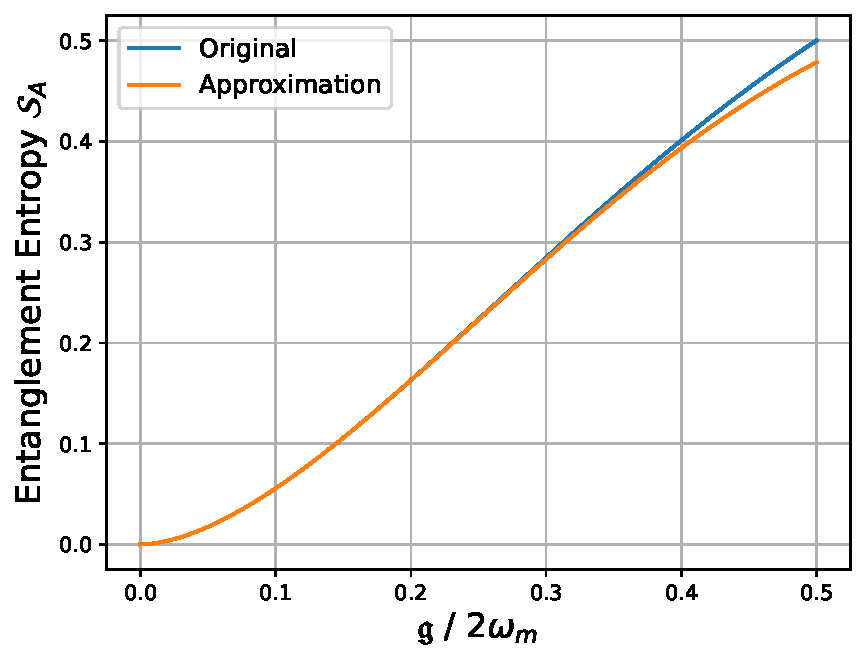
\includegraphics[width=12cm]{EEApprox.pdf}
    \caption{Comparison of the Perturbative Entanglement Entropy and its Approximation.}
    \label{fig: EE1}
\end{figure}
\begin{figure}[htb]
    \centering
    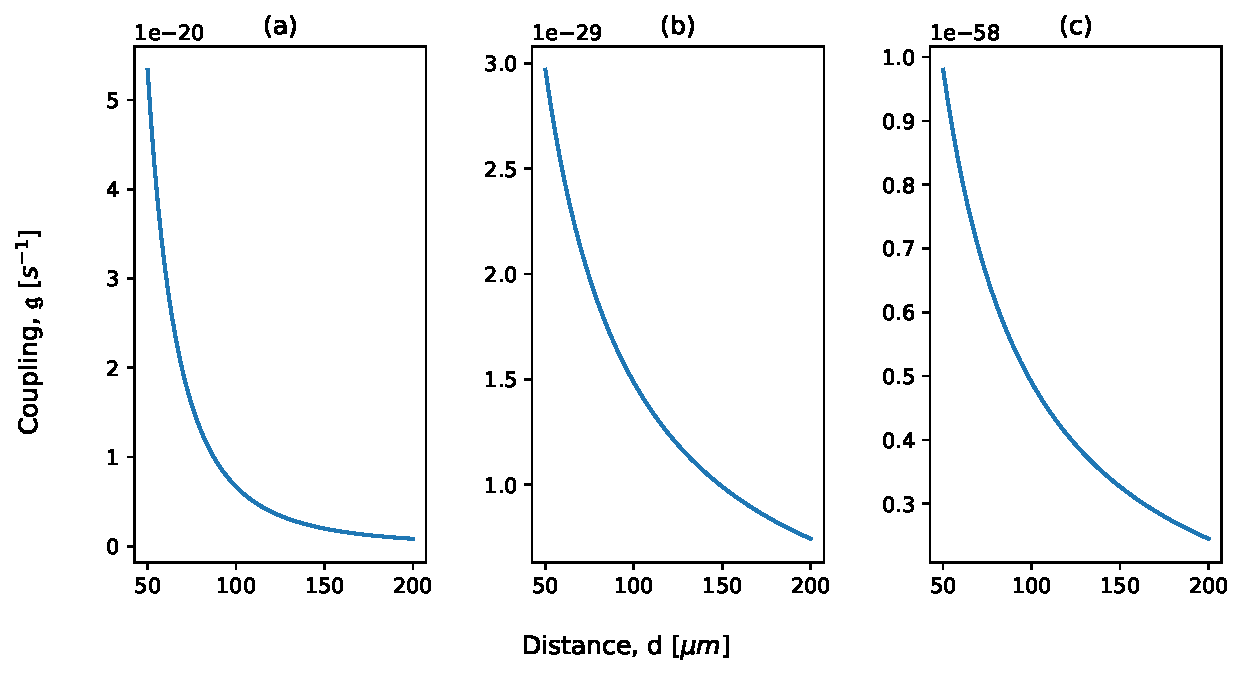
\includegraphics[width=15cm]{Coupling.pdf}
    \caption{Comparison of Coupling for Different Cases:  (a) Static Case; (b) Non-static Correction $1$ (c) Non Static Correction $2$}
    \label{fig:Coupling}
\end{figure}
\begin{figure}[htb]
    \centering
    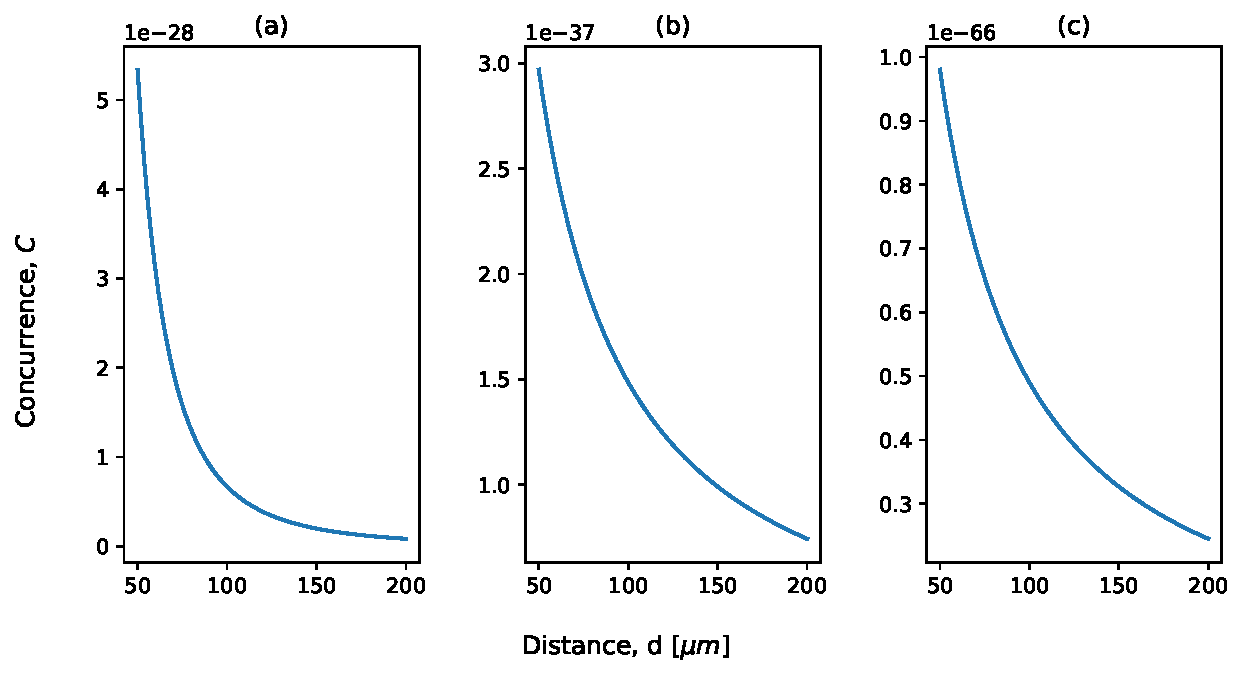
\includegraphics[width=15cm]{ConcCases.pdf}
    \caption{Comparison of Concurrence for Different Cases:  (a) Static Case; (b) Non-static Correction $1$ (c) Non Static Correction $2$}
    \label{fig:Concurrence}
\end{figure}
\begin{figure}[htb]
    \centering
    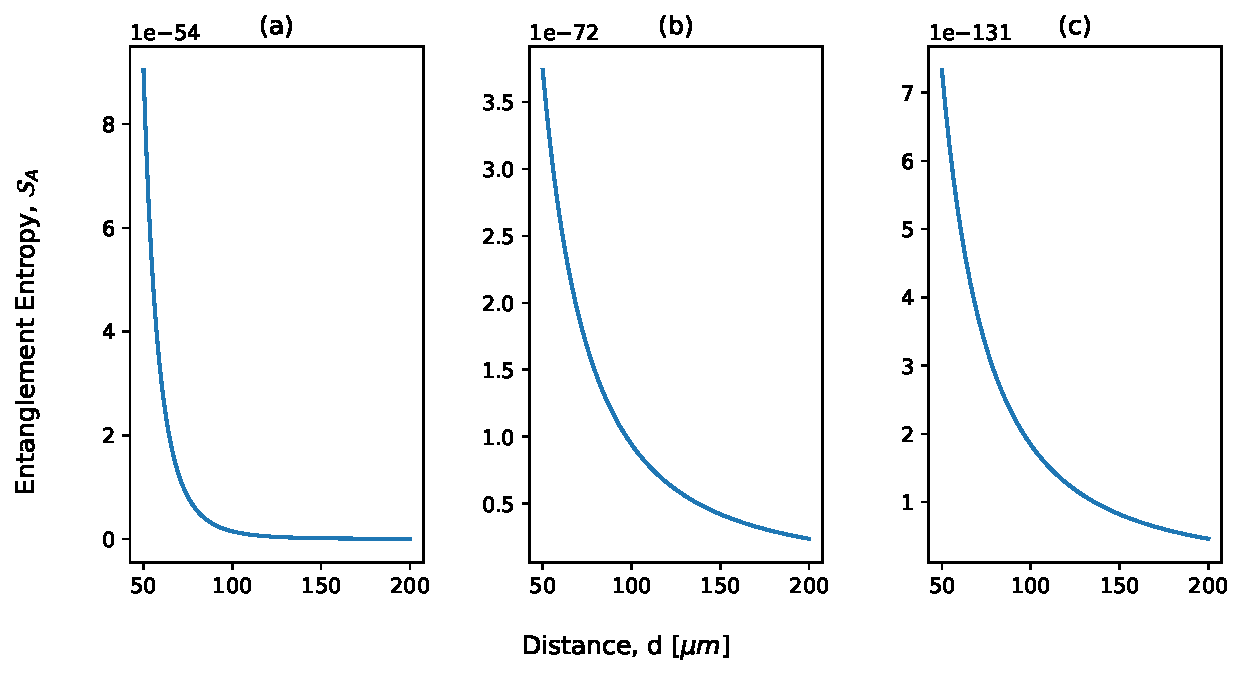
\includegraphics[width=15cm]{EECases.pdf}
    \caption{Comparison of Entanglement Entropies for Different Cases:  (a) Static Case; (b) Non-static Correction $1$ (c) Non Static Correction $2$}
    \label{fig:EE2}
\end{figure}
The code for the visualisation can be found on \url{https://github.com/guprat/MSc_Dissertation}.
\newpage
\chapter{Conclusions}
\newpage
\bibliography{ref}
\newpage
\end{document}